% =====================================================================
%  Minimal_Thesis_Report.tex
%  THE SUBMISSION DOCUMENT: the front matter, six body chapters, the
%  references, and one appendix of complete result tables, generated from
%  artifacts by make_appendix_tables. (No page count is recorded here; it
%  drifts with every edit. Read it off the compiled PDF.)
%
%  Full_Thesis_Report.tex is the 92-page technical version and is retained
%  as a supplement, not as the submission. Both draw every number from the
%  same artifacts in thesis_artifacts/ and both are covered by the
%  304-claim audit in evaluation.audit_numbers, so they cannot disagree.
%
%  Compile with pdfLaTeX, run TWICE (three times after adding a label).
%  Not latexmk: no Perl on the build machine.
% =====================================================================
\documentclass[12pt,a4paper]{report}
\usepackage[left=1.2in,right=0.8in,top=1in,bottom=1in]{geometry}
\usepackage{times}
\usepackage{setspace}
\usepackage{graphicx}
\usepackage{array}
\usepackage{longtable}
\usepackage{booktabs}
\usepackage{float}
\usepackage{amsmath}
\usepackage{amsfonts}
\usepackage{amssymb}
\usepackage{fancyhdr}
\usepackage{titlesec}
\usepackage{tocloft}
\usepackage[hidelinks,hypertexnames=false]{hyperref}
\usepackage[english]{babel}
\usepackage{ragged2e}
\usepackage{parskip}

\renewcommand{\rmdefault}{ptm}
\onehalfspacing

\titleformat{\chapter}[display]
{\normalfont\fontsize{16}{19}\bfseries\centering}
{\chaptertitlename\ \thechapter}{20pt}{\fontsize{16}{19}\bfseries\uppercase}
\titlespacing*{\chapter}{0pt}{10pt}{25pt}
\titleformat{\section}
{\normalfont\fontsize{14}{17}\bfseries}{\thesection}{1em}{}
\titleformat{\subsection}
{\normalfont\fontsize{12}{15}\bfseries}{\thesubsection}{1em}{}

\pagenumbering{roman}
\emergencystretch=3em
\renewcommand{\topfraction}{0.85}
\renewcommand{\bottomfraction}{0.75}
\renewcommand{\textfraction}{0.12}
\renewcommand{\floatpagefraction}{0.90}
\setlength{\cftbeforefigskip}{0pt}
\setlength{\cftbeforetabskip}{0pt}
\setlength{\cftparskip}{0pt}

\begin{document}

% ========================= TITLE PAGE ================================
\begin{titlepage}
\centering
\vspace*{0.5cm}


\includegraphics[width=2.5cm]{images/university logo.jpg}

\vfill

{\fontsize{17}{21}\bfseries
A LIGHTWEIGHT, TRAINING-FREE GEOMETRIC CANONICALIZATION FRAMEWORK FOR CROSS-VIEW COMPARABILITY OF FROZEN MONOCULAR 3D POSE PREDICTIONS
}

\vfill

{\fontsize{14}{17}\selectfont
A PROJECT REPORT
}
\vspace{0.4cm}

{\fontsize{14}{17}\selectfont
Submitted by
}
\vspace{0.4cm}

{\fontsize{16}{19}\selectfont\itshape
MEHEDI HASAN KHAN
}
\vspace{0.3cm}

{\fontsize{14}{17}\selectfont
ID: 12108004 \quad\textbullet\quad Session: 2020-21
}

\vfill

{\fontsize{14}{18}\itshape in partial fulfillment for the award of the degree of\par}
\vspace{0.4cm}

{\fontsize{16}{20} BACHELOR OF SCIENCE IN COMPUTER SCIENCE AND ENGINEERING\par}

\vfill

{\fontsize{14}{18} DEPARTMENT OF COMPUTER SCIENCE AND ENGINEERING\par}

\vfill

{\fontsize{16}{20} COMILLA UNIVERSITY :: COMILLA-3506\par}

\vfill

{\fontsize{14}{18} August 2026\par}
\vspace{0.5cm}

\end{titlepage}

% ===================== BONAFIDE CERTIFICATE ==========================
\newpage
\thispagestyle{empty}
\begin{center}
{\fontsize{18}{22}\bfseries
COMILLA UNIVERSITY :: COMILLA-3506
}
\vspace{1cm}

{\fontsize{16}{19}\bfseries
BONAFIDE CERTIFICATE
}
\end{center}
\vspace{2cm}
\doublespacing
{\fontsize{14}{17}\selectfont
\begin{flushleft}
Certified that this project report titled \textbf{``A Lightweight, Training-Free Geometric Canonicalization Framework for Cross-View Comparability of Frozen Monocular 3D Pose Predictions''} is the bonafide work of \textbf{MEHEDI HASAN KHAN} (ID: 12108004), who carried out the project work under my supervision.
\end{flushleft}
\par}
\singlespacing

\vfill

\noindent
{\fontsize{10}{12}\selectfont
\begin{tabular}{@{}p{0.465\textwidth}c p{0.465\textwidth}@{}}
\rule{7.0cm}{0.5pt} & \hspace{0.2cm} & \rule{7.0cm}{0.5pt} \\
\textbf{SIGNATURE} & & \textbf{SIGNATURE} \\
\textbf{Dr. Md. Faisal Bin Abdul Aziz} & & \textbf{Dr. Mahmudul Hasan} \\
Chairman, Exam Committee & & Supervisor \\
Associate Professor & & Associate Professor \\
Department of Computer Science \& Engineering & & Department of Computer Science \& Engineering \\
Comilla University, Cumilla & & Comilla University, Cumilla \\
\end{tabular}}

\vspace{2cm}

% ============================ ABSTRACT ===============================
\newpage
\setcounter{page}{3}
% \phantomsection before every \addcontentsline: \chapter* creates no hyperref
% anchor, so without it these entries inherit the previous one and the ToC and
% bookmarks jump to the wrong heading.
\phantomsection
\chapter*{ABSTRACT}
\addcontentsline{toc}{chapter}{ABSTRACT}

\doublespacing
{\fontsize{12}{15}\selectfont
Monocular 3D pose estimators express skeletons in the observing camera's frame, so one motion recorded from two viewpoints yields two incomparable sets of coordinates, blocking gait and sports analysis across cameras. Existing remedies retrain the estimator, require calibration, or learn a canonicalization network. We instead build a body-fixed frame from anatomical axes and apply it after prediction, adding no trained parameters to a frozen estimator, and ask what determines whether such a frame stays consistent across viewpoints. On Human3.6M, which played no part in developing the method, canonicalization reduces cross-view distance by 72.2 percent over 180 held-out camera pairs, improving 179 of them. Pose-estimation accuracy is unchanged, because the estimator is frozen: what improves is agreement between cameras, not accuracy against ground truth. A single-view baseline meeting the same requirements, Kabsch alignment to one skeleton, beats our frame on all 180 pairs, and on both backbones no pre-registered search found a regime favouring ours at a corruption severity fixed in advance. The contribution is an experimental boundary rather than a method: axis length governs the choice between frame constructions and nothing finer, articulation rather than radius governs which joint disagrees, and the two alignments fail on disjoint joint supports. A reliability score is falsified as an accuracy predictor across five tests, and a bone-length signal that correlated strongly on one dataset does not replicate on another and is retracted. Seventeen experiments were pre-registered, more than half failed, and every number is re-derived from stored artifacts by an automated audit.
}

\phantomsection
\chapter*{ACKNOWLEDGEMENT}
\addcontentsline{toc}{chapter}{ACKNOWLEDGEMENT}
\justifying
{\fontsize{12pt}{15pt}\selectfont
I would like to express my deepest gratitude to my project supervisor, \textbf{Dr. Mahmudul Hasan}, for his invaluable guidance and continuous support. His requirement to justify every claim against evidence shaped this work: an early evaluation was found to rest on an invalid protocol, and the corrected methodology and audited reporting adopted here follow directly from that. I also thank the Department of Computer Science and Engineering, Comilla University, for the resources and infrastructure, and my family and friends for their constant support.
}

\begin{spacing}{1.0}
\newpage
\tableofcontents
\newpage
% Entry before the list, not after it: placed afterwards the anchor and the
% recorded page are those of the list's last page, not its heading.
\phantomsection
\addcontentsline{toc}{chapter}{LIST OF FIGURES}
\listoffigures
\newpage
\phantomsection
\addcontentsline{toc}{chapter}{LIST OF TABLES}
\listoftables
\end{spacing}

\newpage
\pagenumbering{arabic}
\onehalfspacing

% ========================== CHAPTER 1 ================================
\chapter{INTRODUCTION}
\label{ch:intro}

\begin{figure}[htbp]
\centering
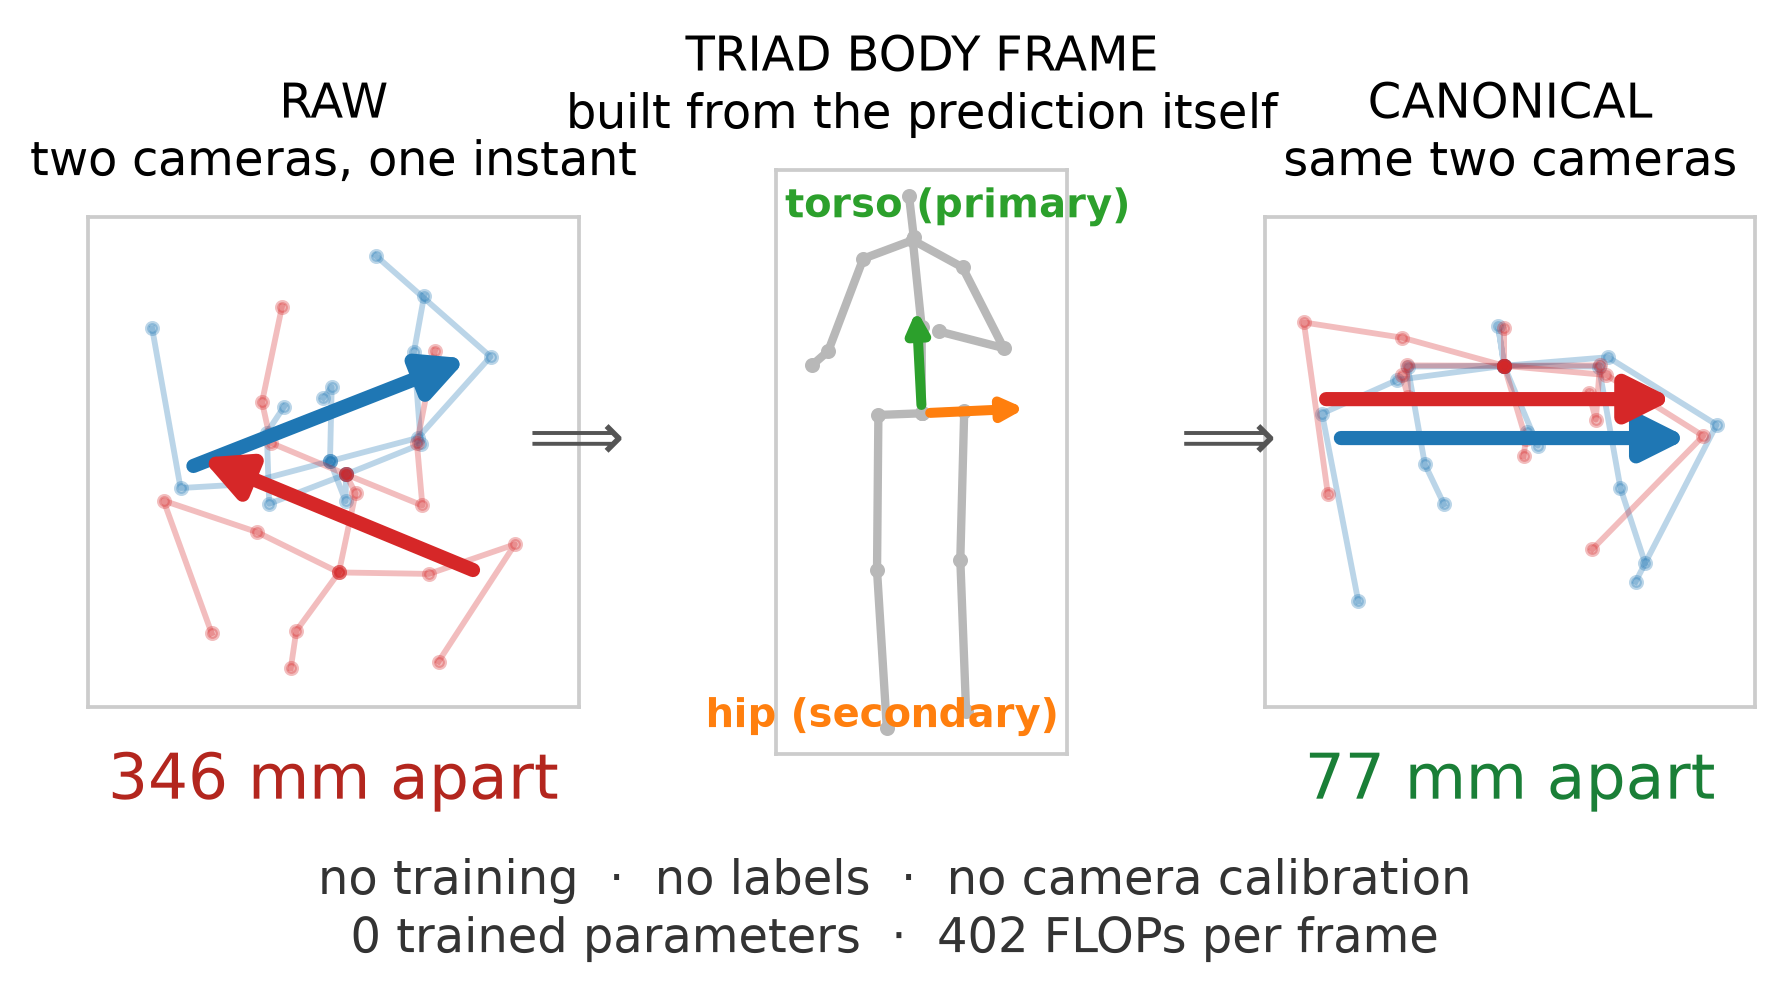
\includegraphics[width=\textwidth]{images/fig_teaser.png}
\caption[The problem and the operation]{The problem and the operation, on one instant of Human3.6M seen by two synchronized cameras. Left and right are drawn from above, because two views of the same instant differ mainly in azimuth. All three panels are real predictions and the distances are the measured ones.}
\label{fig:teaser}
\end{figure}

\section{Background}

Three-dimensional human pose estimation aims to recover the spatial coordinates of human body joints from visual input. Among the available approaches, monocular 3D pose estimation from a single RGB camera is especially attractive because it requires only inexpensive and widely available imaging devices. Recent transformer-based lifting models, including MotionAGFormer \cite{motionagformer} and MotionBERT \cite{motionbert}, report low mean per-joint position errors on the Human3.6M benchmark \cite{h36m}, demonstrating that high-quality 3D pose estimation is now possible from ordinary monocular video.

A single image, however, does not determine a 3D pose. Perspective projection maps a whole family of skeletons, differing in depth and in overall scale, onto the same image coordinates, so recovering one of them requires assumptions about human proportion and articulation rather than measurement alone. Martinez et al.~\cite{martinez} showed that this residual ambiguity, rather than image feature extraction, is where the difficulty of the task concentrates. Modern estimators resolve it statistically, from what human bodies typically look like and how they typically move. Their accuracy is not what this thesis sets out to change; the estimator used here is frozen throughout.

Despite their strong accuracy, these models share an important limitation. Their predicted poses are represented in the coordinate system of the observing camera. Consequently, two synchronized cameras capturing the same person at the same instant produce different coordinate representations of an identical physical pose. This viewpoint dependency makes direct comparison across cameras impossible without first transforming the predictions into a common reference frame. Such a capability is essential in applications including gait analysis across recording sessions, sports performance analysis from multiple camera positions, and other cross-view motion analysis tasks. Such a frame is constrained in three ways by the setting in which it must operate. It has to be derivable from the prediction itself, because camera parameters are unavailable; it has to rotate with the subject, so that two views of one pose yield one representation; and it must be obtainable without modifying or retraining the estimator that produced the prediction.

This thesis studies such a frame under exactly those constraints, and measures it where two synchronized cameras observe the same instant, a setting in which agreement between views can be measured without any ground truth at all. Figure~\ref{fig:teaser} shows this viewpoint dependency, and the operation applied to it in this work, on two synchronized views of a single instant.

\section{Motivation}

This work is motivated by three practical deployment constraints.

First, retraining the underlying pose estimator is often infeasible. In many real-world settings, the model is a frozen third-party component, labeled training data is unavailable, and the computational resources required for retraining are impractical.

Second, accurate camera calibration cannot always be assumed. Many applications rely on videos collected from consumer devices or uncontrolled environments where intrinsic and extrinsic camera parameters are unknown.

Third, reliability is as important as accuracy. A system that confidently produces an incorrect pose can be more harmful than one that acknowledges uncertainty. Therefore, a practical canonicalization framework should not only improve cross-view consistency but also provide an indication of when its output should not be trusted.

\section{Research Question and Objectives}
\label{sec:rq}

This project is guided by the following research question:

\begin{quote}
\textbf{What determines whether an anatomical reference frame remains consistent across viewpoints?}
\end{quote}

The proposed framework is not the primary contribution but rather the means of investigating this question. By constructing a lightweight body-fixed reference frame that operates on a frozen pose estimator without retraining, camera calibration, or additional supervision, all other variables can be held constant. This isolation allows the consistency of the reference frame itself to be studied directly. Figure~\ref{fig:architecture} shows where this stage sits relative to the frozen components it is applied to. Everything above the dashed line is trained by its authors and used here frozen and unmodified; everything below it is this work, and it adds no trained parameters, consumes no labels and uses no camera parameters. The identity beneath the diagram is why: the frame is built from the joints, so it rotates with them, and the unknown rotation between two cameras cancels rather than being estimated.

The objectives of this work are fourfold. First, to construct a viewpoint-independent coordinate frame that operates on the outputs of a frozen monocular 3D pose estimator without requiring training, labeled data, or camera parameters. Second, to identify the design factor that governs cross-view consistency and determine the conditions under which the derivation remains valid, as well as its limitations. Third, to develop an analytical reliability score that enables the system to abstain when the estimated frame is unreliable. Finally, to evaluate the framework under a fully auditable experimental protocol in which every reported result can be reproduced automatically from stored artifacts.

\begin{figure}[htbp]
\centering
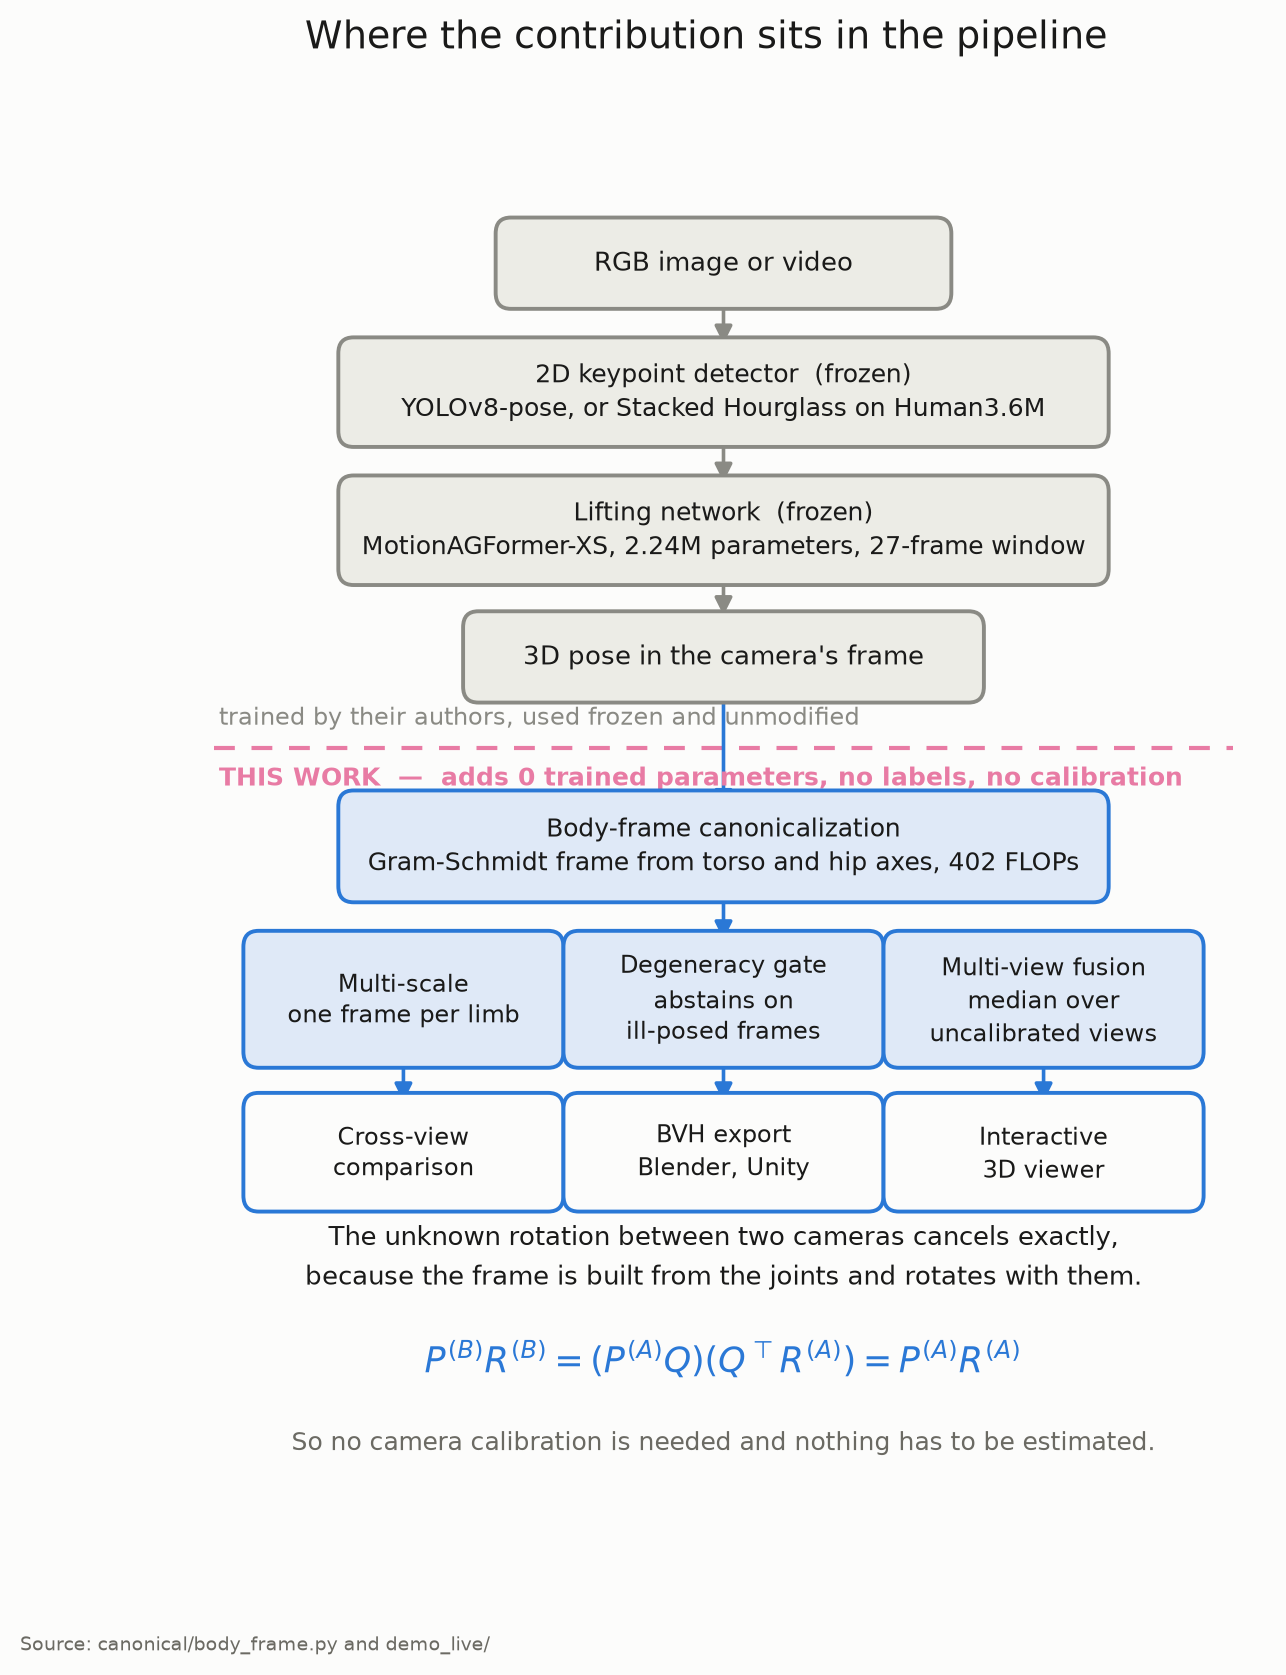
\includegraphics[width=\textwidth]{images/fig_architecture.png}
\caption[Where the contribution sits in the pipeline]{Where the contribution
sits in the pipeline. Everything above the dashed line is frozen; everything
below it is this work.}
\label{fig:architecture}
\end{figure}

\section{Contributions}

The geometric foundations used in this work are not original. The reference frame is based on the TRIAD algorithm \cite{triad}, the primary-axis selection follows the method of Shuster and Oh \cite{shuster}, and the propagation of landmark error into frame orientation is established in biomechanics \cite{dellacroce1999,dellacroce2005}. Our contribution lies in applying these principles to joint predictions produced by a frozen monocular 3D pose estimator and, more importantly, in experimentally establishing the limits of their applicability.

The main contributions of this thesis are summarized below.

\begin{itemize}
\item \textbf{Analysis.} We identify the axis-length principle as the key factor governing the choice between reference-frame constructions, while showing that joint disagreement is primarily determined by articulation rather than axis length.

\item \textbf{Validation.} We demonstrate cross-view consistency on the Human3.6M benchmark, where canonicalization improves cross-view distance for 179 of 180 held-out camera pairs without retraining, camera calibration, or additional supervision.

\item \textbf{Empirical finding.} We show that the proposed reliability score is not a reliable predictor of pose accuracy but is effective as a confidence measure for deciding when canonicalization should be trusted.

\item \textbf{Negative result.} We demonstrate that a temporal bone-length signal, which appeared promising on one dataset, does not generalize across datasets and is therefore rejected as a reliable indicator.

\item \textbf{Engineering contribution.} We develop a calibration-free multi-view fusion strategy and show that the choice of aggregation statistic, specifically the mean versus the median, determines whether combining multiple views is beneficial.

\item \textbf{Systems contribution.} We build a fully reproducible evaluation framework spanning two datasets and two frozen backbone architectures. The evaluation includes cross-dataset replication, 304 audited claims automatically re-derived from stored artifacts, 76 passing verification tests, and 17 pre-registered experiments with transparent reporting of both successful and unsuccessful outcomes.
\end{itemize}

\paragraph{Position of this work.} Existing research has studied anatomical canonicalization, geometric alignment, and reliability estimation separately. This thesis brings these three components together within a single post-processing framework that operates on frozen monocular 3D pose estimators. The framework is evaluated across two datasets, two backbone architectures, and a series of pre-registered boundary experiments. The literature reviewed in Chapter~\ref{ch:related} does not identify previous work investigating this combination under the simultaneous constraints of requiring no retraining, no labeled data, and no camera calibration.

\section{Report Organization}

The remainder of this thesis is organized as follows. Chapter~\ref{ch:related} reviews the relevant literature and positions the proposed work within the existing body of research. Chapter~\ref{ch:method} presents the proposed methodology. Chapter~\ref{ch:data} describes the datasets, evaluation protocol, and experimental setup. Chapter~\ref{ch:results} reports the experimental results, including negative findings, the post-freeze failure-support analysis, and the routing rule. Finally, Chapter~\ref{ch:conclusion} concludes the thesis and discusses future directions.

% ========================== CHAPTER 2 ================================
\chapter{LITERATURE REVIEW}
\label{ch:related}

\section{Monocular 3D Pose Estimation}

Modern monocular 3D human pose estimation pipelines typically follow a two-stage architecture. A 2D keypoint detector first identifies body joints in the image, after which a lifting network reconstructs their corresponding 3D coordinates. This separation remains effective because the two stages fail for different reasons: the detector is primarily affected by occlusion and motion blur, whereas the lifting stage must resolve the inherent depth ambiguity of monocular images. Martinez et al.~\cite{martinez} demonstrated that a simple network consisting of two residual blocks, when provided with ground-truth 2D keypoints, outperformed contemporary end-to-end image-based methods. Their results established that much of the challenge lies in the 2D-to-3D lifting problem rather than in image feature extraction.

Subsequent research focused on exploiting temporal information to reduce depth ambiguity. This led to sequence-based models such as VideoPose3D \cite{videopose}, which uses dilated temporal convolutions, and transformer-based approaches including MotionBERT \cite{motionbert} and MotionAGFormer \cite{motionagformer}. MotionAGFormer combines transformer and graph-convolutional streams, and its extra-small variant, MotionAGFormer-XS, achieves an MPJPE of 45.1~mm on the Human3.6M benchmark while using only 2.2 million parameters. MotionAGFormer-XS is used as the frozen backbone throughout this work.

Two observations are particularly relevant to this thesis. First, reported benchmark accuracy represents an average performance and can vary substantially across different human actions. Second, existing methods express predicted poses in the coordinate system of the observing camera, making direct comparison across viewpoints impossible. Consequently, estimation accuracy and cross-view comparability are distinct properties, and improvements in one do not automatically lead to improvements in the other.

\section{Canonicalization and View-Invariant Representations}

Several previous studies have addressed viewpoint dependence in monocular 3D pose estimation. Among them, 3DPCNet \cite{3dpcnet} is the closest to the present work. It performs estimator-agnostic pose canonicalization using a neural network trained on synthetically rotated poses, and evaluates a handcrafted anatomical-landmark baseline that is conceptually similar to ours. Their learned model achieves approximately six times lower rotation error than the handcrafted alternative. Rather than overlooking this result, we use it as an important point of comparison and discuss its implications in Section~\ref{sec:positioning}.

Other approaches also rely on learning-based representations. MoViD \cite{3dpcnet2} disentangles motion from viewpoint through an orthogonal projection learned under SMPL \cite{smpl} supervision. V-VIPE \cite{vvipe} learns a variational view-invariant embedding and applies Kabsch alignment using the hip and spine joints as preprocessing. Wei et al.~\cite{vihc} transform predicted poses into a common coordinate system before refining them with a learned network and discriminator. Although these methods differ in architecture, they all require training, supervision, or both. In contrast, the distinguishing feature of the present work is not the underlying geometry itself, but the deployment setting: a frozen pose estimator operating without retraining, labeled data, or camera calibration.

A separate and much older line of work aligns two point sets directly. Given corresponding points, the rotation minimizing squared distance between them has a closed-form solution \cite{kabsch}, and this requires neither training nor calibration. Aligning every predicted skeleton to one fixed reference skeleton therefore produces a viewpoint-independent representation by the same means, and V-VIPE uses exactly this as preprocessing \cite{vvipe}. This alignment satisfies the same deployment constraints as the anatomical frame studied here, and Chapter~\ref{ch:results} reports it as the stronger of the two on the headline metric.

\section{Quality and Uncertainty Estimation for Pose}

For a pose estimation system to abstain from unreliable predictions, it must estimate the confidence of its own output. Existing approaches generally fall into three categories.

The first category consists of learned uncertainty estimation, where additional prediction heads or ensembles are trained to estimate model error. Khanal and Zhou \cite{khanal} describe an important limitation of such approaches in the related task of skeleton-based action recognition. Under severe domain shift, energy-based methods successfully detect distribution changes while the model remains confidently incorrect on individual predictions.

The second category is conformal prediction \cite{yangpavone}, which provides statistical coverage guarantees but requires a labeled calibration dataset drawn from the deployment distribution.

The third category uses analytic, training-free confidence measures based on geometric consistency. Because these methods require neither retraining nor labeled deployment data, they are particularly attractive for frozen models. This work adopts an analytic approach. As shown in Chapter~\ref{ch:results}, however, the proposed reliability measure does not accurately predict pose error, although it remains useful for determining when canonicalization should be trusted.

\section{What This Work Inherits From Attitude Determination}

Constructing an orthonormal reference frame from two measured directions by selecting one as the primary axis, orthogonalizing the second, and obtaining the third through a cross product is the basis of the TRIAD algorithm introduced by Black \cite{triad} in 1964. Shuster and Oh \cite{shuster} later showed that the most reliable direction should be chosen as the primary axis and that orientation accuracy is maximized when the measured directions are nearly orthogonal. For more than two observations, Wahba's problem \cite{wahba} provides the corresponding least-squares formulation, whose optimality depends on inverse-variance weighting.

The uncertainty of a direction estimated from two joints separated by a distance $L$, each affected by measurement noise $\sigma$, is approximately $2\sigma/L$. The propagation of landmark uncertainty into anatomical reference-frame orientation has been studied extensively in biomechanics \cite{dellacroce1999,dellacroce2005}. This thesis applies these established geometric principles to joint coordinates predicted by frozen neural networks and investigates the conditions under which they remain effective.

Table~\ref{tab:requirements} summarizes the deployment requirements of representative approaches.

\begin{table}[H]
\centering
\caption{Requirements of related approaches at deployment time}
\label{tab:requirements}
\small
\begin{tabular}{|l|c|c|c|c|}
\hline
\textbf{Method} & \textbf{Training} & \textbf{Labels} & \textbf{Camera params} & \textbf{Multi-view input} \\
\hline
MoViD \cite{3dpcnet2} & Required & GT SMPL & No & No \\
\hline
3DPCNet \cite{3dpcnet} & Required & Synthetic rotations & No & No \\
\hline
V-VIPE \cite{vvipe} & Required & 3D ground truth & No & No \\
\hline
Conformal \cite{yangpavone} & None & Labeled calibration set & No & No \\
\hline
\textbf{This work} & \textbf{None} & \textbf{None} & \textbf{None} & Optional \\
\hline
\end{tabular}
\end{table}

\section{Multi-View Fusion}

Classical multi-view pose estimation triangulates 2D detections using known
camera calibration, which yields excellent accuracy and requires the
calibration. CMANet \cite{cmanet} learns a canonical space for multi-view 3D pose without
manual 3D annotation, supervising itself from the confident outputs of an
existing 2D detector, and V-VIPE learns a variational view-invariant embedding
that supports retrieval across viewpoints. Both require training, and CMANet
additionally requires several views at inference rather than only during
training.

The gap this project occupies is fusion when calibration is unavailable and
training is not an option. If predictions from several cameras can be placed in a
shared frame by construction, they can be combined by simple statistics without
correspondence search or extrinsics. Chapter~\ref{ch:results} reports that this
works, and that the statistic must be robust when the views are few.

\section{Positioning of This Work, and the Closest Prior Baseline}
\label{sec:positioning}

No prior method operates on a frozen estimator with no training, no labels and no
camera parameters simultaneously. That requirement profile, rather than any
individual mechanism, is the position this project occupies. Geometric
canonicalization itself is not claimed here as novel, and the specific
construction is more thoroughly trodden than a single comparison would suggest.

\textbf{One prior result bears directly against this work and is stated here
rather than left for a reader to find.} 3DPCNet \cite{3dpcnet}, published at ICASSP 2026,
addresses the same problem with a learned self-supervised module, and includes a
hand-built geometric baseline of the same family as ours: it defines a plane from
the shoulder and hip joints, aligns that plane's normal to a fixed axis, and then
aligns the shoulder vector to a second axis. That is a two-vector attitude
construction of the TRIAD family. Their Table 1 reports it at \textbf{20.6
degrees of rotation error against 3.58 degrees} for their learned module, on the
MM-Fi dataset \cite{mmfi}. The anatomical family is therefore not unmeasured in the
literature; it is measured, and characterised as inferior to a learned
alternative.

Four qualifications apply, and none of them overturns that result. Their MPJPE
column is confounded by their own admission, because their module makes non-rigid
shape edits the geometric baseline never attempts, so only the rotation column is
a clean comparison. It is the proposing authors' own implementation of a
competitor, in a single table without error bars, seeds or an oracle upper bound.
It measures alignment against a ground-truth canonical pose, whereas this report
measures agreement between two cameras, which is a different quantity. And its
primary axis is the shoulder-hip plane normal, which is not the construction used
here, so the correct description is same-family rather than identical. The
direction of their finding nevertheless agrees with the baseline comparison of
Chapter~\ref{ch:results}, and it is more honest to say that the evidence points
the same way twice than to argue either result away.

Closer still, Wei et al. \cite{vihc} transform predicted poses into consistent views before
refining them, first at the global body level and then at the level of local body
parts, which is the same two-level decomposition this report arrives at, from the
same anatomical landmarks. What differs is not the geometry but everything around
it: their transformation feeds a trained correction network and a trained
discriminator, so it is unavailable to a practitioner who cannot train, and the
consistent views are an intermediate step rather than a quantity they evaluate.

The contribution is therefore not the construction but the requirement profile
that keeps it usable on a frozen estimator, and the experimental boundary that
follows. The construction is treated as an instrument rather than as a result: a
frame with no trained parameters and no calibration allows every variable except
the frame's own construction to be held fixed, and that is what makes the
boundary measurable.

\subsection{Research Gap}
\label{sec:gap}

The approaches reviewed above resolve viewpoint dependence in three ways, and each
carries a deployment cost. Learned canonicalization \cite{3dpcnet,3dpcnet2,vvipe,vihc}
requires training and supervision. Calibrated multi-view triangulation requires camera
parameters. Conformal methods \cite{yangpavone} require a labeled calibration set drawn
from the deployment distribution. Table~\ref{tab:requirements} summarizes these
requirements side by side.

The literature reviewed here does not identify a method that combines the constraints of
requiring no retraining, no labeled data and no camera calibration while operating as a
post-processing stage on a frozen pose estimator. That unaddressed combination, a
requirement profile rather than a mechanism, is the gap this thesis occupies, and it is
what makes the research question of Section~\ref{sec:rq} answerable: with no trained
parameters and no calibration anywhere in the pipeline, every variable except the frame's
own construction can be held fixed.

The gap is one of deployment setting, not of geometry. The construction itself is not
new, and Section~\ref{sec:positioning} has already reported a published result in which a
same-family construction is measured and characterised as inferior to a learned
alternative.

% ========================== CHAPTER 3 ================================
\chapter{METHODOLOGY}
\label{ch:method}

\section{Scope of the Term Training-Free}

The complete pose estimation pipeline is not training-free. Both the 2D keypoint detector \cite{yolov8} and the 3D lifting network \cite{motionagformer,motionbert} are pretrained models developed by their respective authors and are used here without modification. The term \emph{training-free} refers only to the components introduced in this work.

More precisely, the claim concerns the deployment requirements rather than the history of the pipeline. Applying the proposed framework to a different pose estimator requires no additional training data, labeled examples, camera calibration, or gradient-based optimization. This claim would be invalidated if the framework required dataset-specific tuning. The strongest evidence against that possibility is provided by the Human3.6M evaluation, where all constants were fixed on MPI-INF-3DHP \cite{mpi} and applied unchanged to 180 previously unseen camera pairs \cite{h36m}.

\section{Body-Frame Canonicalization}

\begin{figure}[H]
\centering
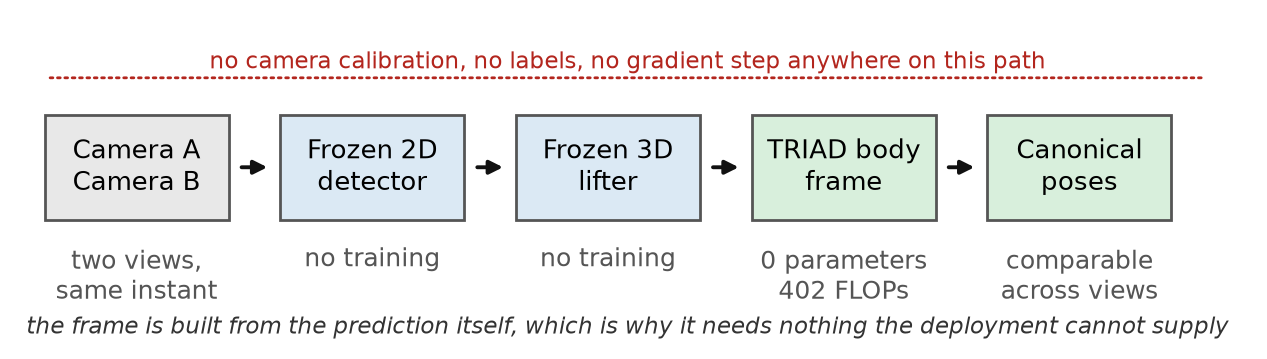
\includegraphics[width=\textwidth]{images/fig_pipeline.png}
\caption[The pipeline end to end]{The pipeline end to end: RGB video, a frozen 2D detector, conversion to the Human3.6M joint layout, a frozen lifter, and the canonicalization this thesis adds.}
\label{fig:pipeline}
\end{figure}


Figure~\ref{fig:pipeline} shows the pipeline end to end; the final stage is the
only one this work adds. Let $P \in \mathbb{R}^{17\times 3}$ be a root-relative predicted pose in the H36M-17 joint convention \cite{h36m}. We construct a body-fixed orthonormal frame as
\begin{align}
\mathbf{y} &= \frac{P_{8} - P_{0}}{\lVert P_{8} - P_{0} \rVert}, \qquad
\mathbf{x}_{\text{raw}} = P_{1} - P_{4}, \\
\mathbf{z} &= \frac{\mathbf{x}_{\text{raw}} \times \mathbf{y}}{\lVert \mathbf{x}_{\text{raw}} \times \mathbf{y} \rVert},
\qquad
\mathbf{x} = \mathbf{y} \times \mathbf{z}, \\
R &= [\,\mathbf{x} \mid \mathbf{y} \mid \mathbf{z}\,], \qquad
P_{\text{can}} = P R .
\end{align}
Here $\mathbf{y}$ is the torso vertical axis (pelvis to thorax, joints 0 and 8) and $\mathbf{x}_{\text{raw}}$ the hip axis (right hip to left hip, joints 1 and 4). The construction is closed form, costs $O(17)$ operations per frame, and has no free parameters. It is TRIAD \cite{triad} with the torso axis primary, named rather than claimed. The construction is deliberately asymmetric: $\mathbf{y}$ is reproduced exactly while $\mathbf{x}_{\text{raw}}$ influences only the rotation about it, so the choice of primary axis is a design decision, and the established guidance \cite{shuster} is to make the more accurately known direction primary---for a skeleton, the longer segment.

\subsection{Why This Construction Achieves View Invariance}

\begin{figure}[H]
\centering
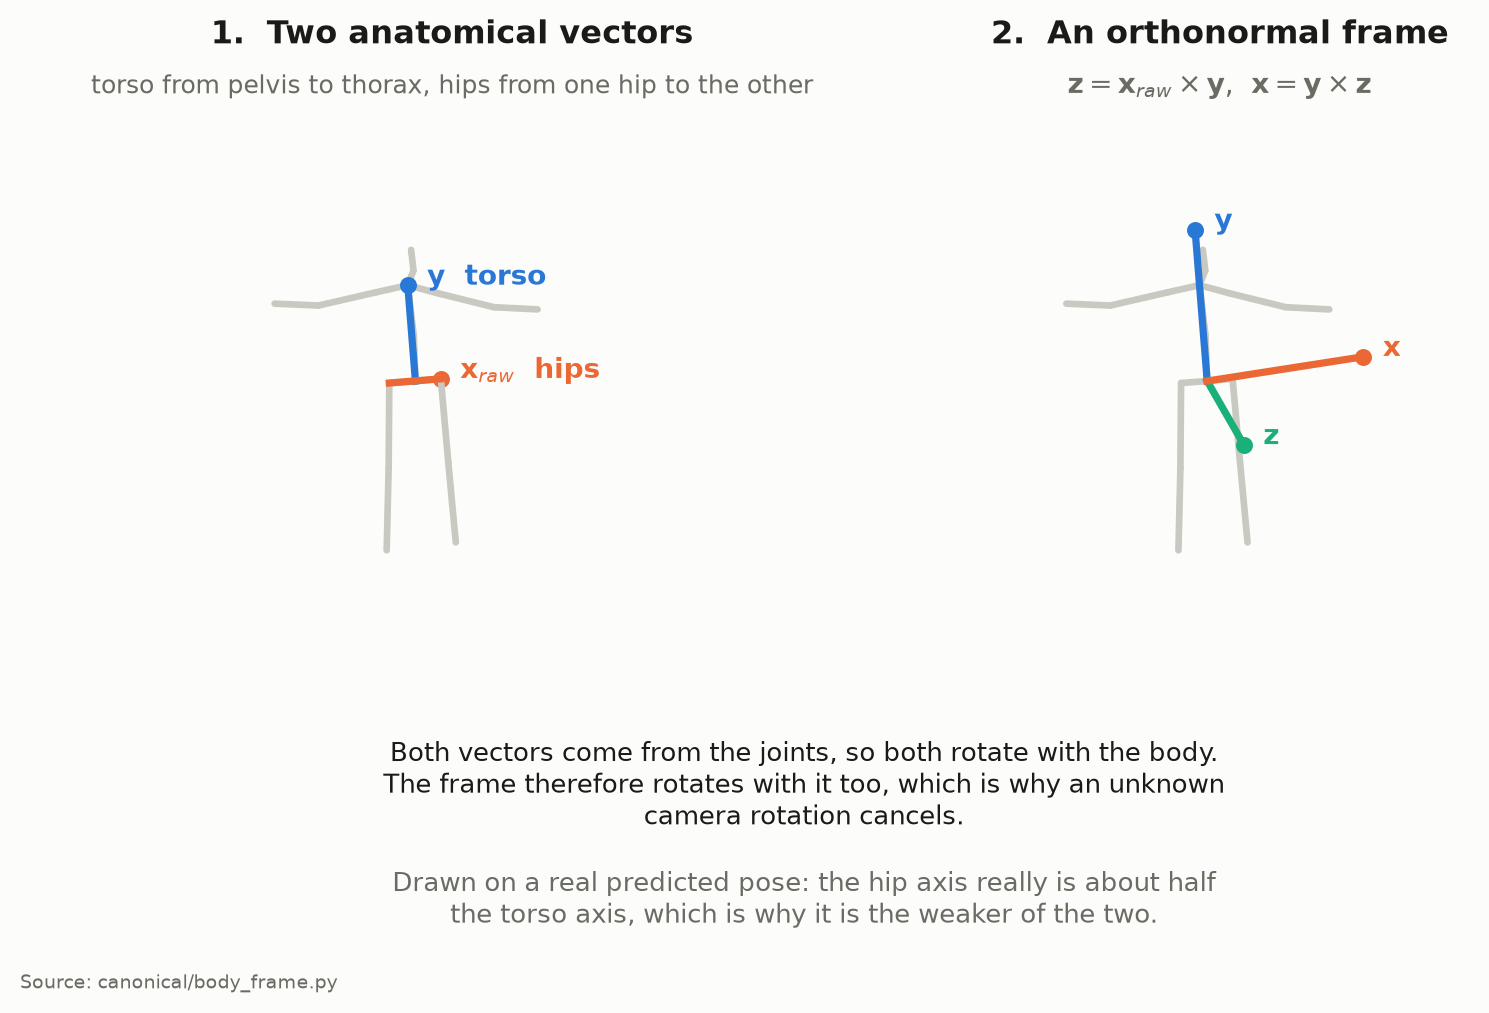
\includegraphics[width=\textwidth]{images/fig_frame_construction.png}
\caption[The body-frame construction]{The frame construction: the torso axis from pelvis to thorax, the hip axis between the hips, and Gram-Schmidt orthonormalization.}
\label{fig:framecon}
\end{figure}


Figure~\ref{fig:framecon} illustrates the construction and the cancellation that
follows from it. Suppose cameras $A$ and $B$ observe one configuration, so their root-relative predictions are related by an unknown rotation, $P^{(B)} = P^{(A)} Q$ for some $Q \in SO(3)$. Because the axes are built from the joint positions themselves, each axis rotates with the pose, so the frames satisfy $R^{(B)} = Q^{\top} R^{(A)}$, and
\begin{equation}
P^{(B)}_{\text{can}} = P^{(B)} R^{(B)} = \left(P^{(A)} Q\right)\left(Q^{\top} R^{(A)}\right) = P^{(A)}_{\text{can}} .
\end{equation}
The unknown rotation cancels exactly, without ever being estimated. This is why no calibration is required. The argument is exact only when both cameras yield the same pose up to rotation; in practice each prediction carries its own error, and the residual canonical distance we measure is precisely that term.

\subsection{Why Axis Length Governs Frame Stability}

Suppose a direction is estimated from two predicted joints separated by distance $L$, each carrying independent isotropic position noise of standard deviation $\sigma$. The segment vector carries variance $2\sigma^2$ per component; only the perpendicular component rotates it, with two degrees of freedom, so for small angles the induced angular error is
\begin{equation}
\theta_{\mathrm{rms}} \;\approx\; \frac{2\sigma}{L} .
\label{eq:theta}
\end{equation}
Angular error is inversely proportional to segment length. Propagating to the measured quantity---a frame in error by $\theta$ displaces a joint at radius $r$ by roughly $r\theta$, and two views combine in quadrature---gives
\begin{equation}
d^{2} \;\approx\; \Big(c\,\frac{\bar{r}}{L}\Big)^{2} + d_0^{2},
\label{eq:axislaw}
\end{equation}
where $d$ is the mean cross-view joint distance, $\bar{r}$ the mean of $r$ over
the scored joints, $c = 2\sqrt{2}\,\sigma$ the constant carrying the keypoint
noise scale together with the two-view quadrature factor, and $d_0$ the part of
the disagreement that does not come from the frame at all. The two constants $c$
and $d_0$ are fitted rather than assumed. Equation~\eqref{eq:axislaw} is
falsifiable and is tested in Section~\ref{sec:axisboundary}.

\subsection{Degeneracy Handling}

Three degenerate configurations are detected explicitly and treated as invalid rather than producing potentially misleading outputs.

\begin{itemize}
\item The torso axis is shorter than 5\% of the median bone length.
\item The hip axis is nearly parallel to the torso axis.
\item The constructed reference frame fails the orthonormality check.
\end{itemize}

Frames satisfying any of these conditions are excluded from all aggregate analyses. On the Human3.6M dataset, however, none of these degeneracies occurred, and the construction was valid for every evaluated frame.

\section{Analytic Reliability Score}

The proposed reliability score is computed entirely from the predicted pose without requiring ground-truth annotations or additional training. Six geometric indicators are evaluated:

\begin{itemize}
\item axis conditioning,
\item the torso--hip angle,
\item bilateral symmetry of limb lengths,
\item the fraction of anatomically abnormal bone-length ratios,
\item the minimum detector keypoint confidence, and
\item temporal stability of the body frame.
\end{itemize}

Each indicator is normalized to the interval $[0,1]$ using fixed constants and combined through a geometric mean, ensuring that a single severely degraded component drives the overall score toward zero. In addition, four hard geometric validity checks trigger abstention regardless of the combined score.

As shown in Chapter~\ref{ch:results}, this reliability score does not accurately predict pose estimation error. The reason is structural rather than empirical: every component is computed solely from the geometry of a single predicted skeleton. Consequently, a pose that is incorrect primarily along the depth dimension may still appear anatomically plausible, well-conditioned, symmetric, and proportionally consistent, resulting in a high reliability score despite a large reconstruction error.

\section{Calibration-Free Multi-View Fusion}

Once canonicalization expresses the predictions from all cameras in a common body-fixed reference frame, poses from multiple uncalibrated viewpoints become directly comparable. This enables multi-view fusion without estimating camera extrinsics, performing correspondence search, or requiring camera calibration.

Three aggregation strategies are evaluated: the unweighted mean, the reliability-weighted mean, and the coordinate-wise median. The choice of aggregation function is important because these estimators differ in robustness to outliers. The arithmetic mean has a breakdown point of zero \cite{hampel}, meaning that even a single severely corrupted prediction can substantially influence the result. In contrast, the coordinate-wise median remains stable until nearly half of the input views become unreliable. As demonstrated in Section~\ref{sec:fusion}, this difference determines whether multi-view fusion improves or degrades performance when only a small number of camera views are available.

\section{Temporal Bone-Length Inconsistency}

Human bone lengths remain effectively constant over time. Consequently, temporal variation in predicted bone lengths provides a geometric indicator of pose estimation error.

For each frame, the sixteen bone lengths are normalized by the mean bone length of that frame to remove scale variation. A label-free reference skeleton is then estimated as the median normalized skeleton over a temporal window. The temporal inconsistency signal is defined as the mean relative deviation of the current normalized bone lengths from this reference.

% ========================== CHAPTER 4 ================================
\chapter{DATASETS AND EVALUATION PROTOCOL}
\label{ch:data}

\section{MPI-INF-3DHP}

MPI-INF-3DHP \cite{mpi} is a multi-camera markerless motion capture dataset recorded with fourteen synchronized cameras. This work uses subjects S1 and S2 under both static and dynamic recording conditions, which are treated as separate evaluation strata throughout the experiments.

A total of twenty-nine camera pairs are considered. One pair is reserved exclusively for method development and parameter selection, twenty-seven pairs are held out on subject S1, and one additional pair is reserved for the unseen subject S2. MPI-INF-3DHP therefore serves as the development dataset, where all algorithmic constants are determined before validation.

\section{Human3.6M}

\begin{figure}[htbp]
\centering
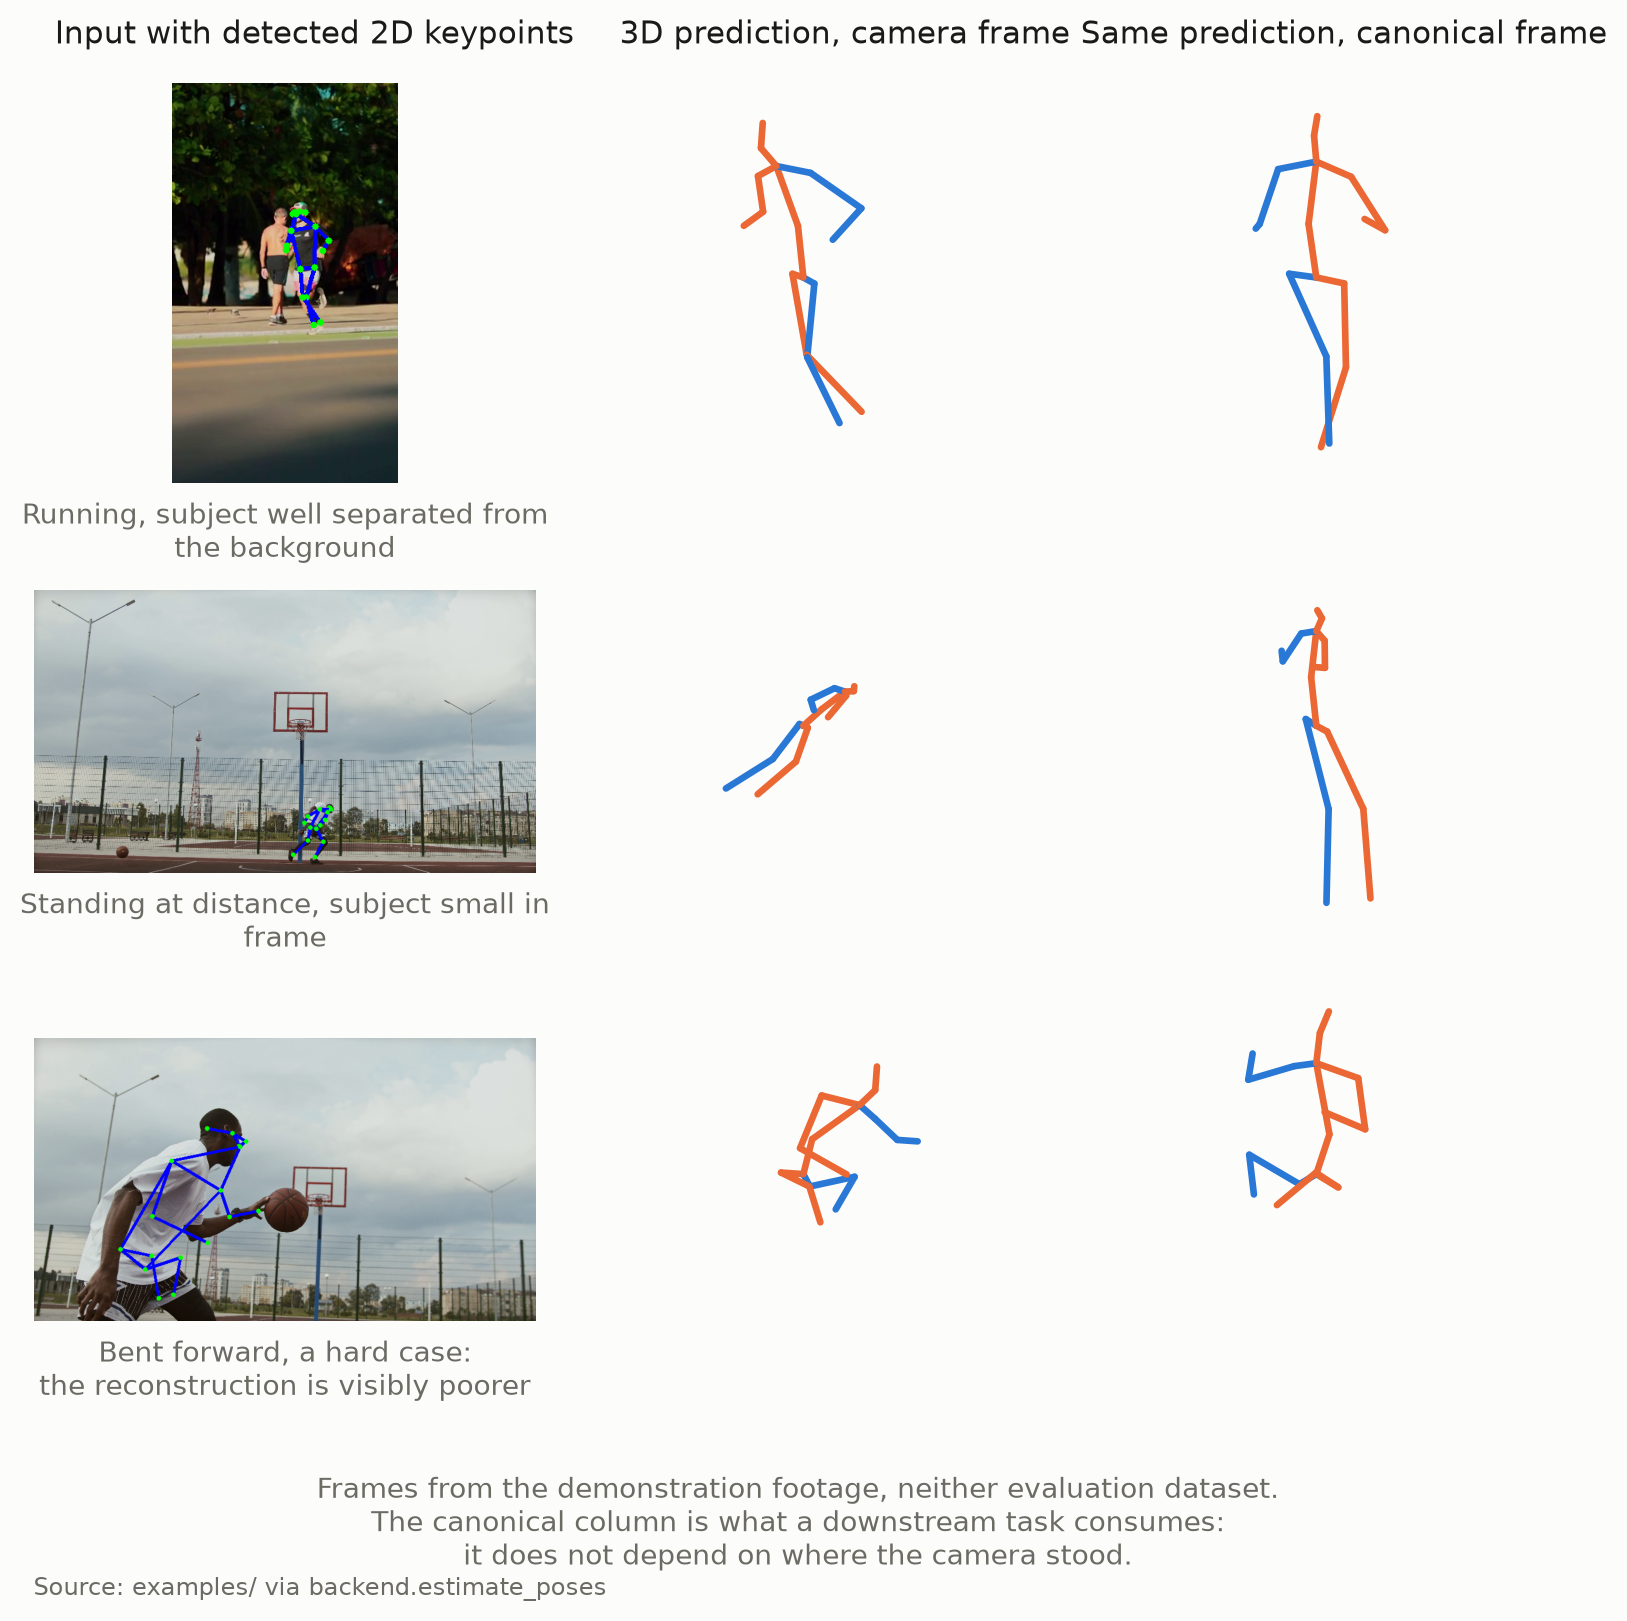
\includegraphics[width=\textwidth]{images/fig_qualitative.png}
\caption[The pipeline on uncontrolled footage]{The pipeline on uncontrolled footage, outside either evaluation dataset. Left: the input frame with the detected 2D keypoints. Middle: the lifted 3D prediction in the camera's frame. Right: the same prediction after canonicalization.}
\label{fig:qualitative}
\end{figure}


Human3.6M \cite{h36m} is the standard benchmark for monocular 3D human pose estimation. It contains eleven subjects performing fifteen activities, recorded simultaneously by four synchronized cameras operating at fifty frames per second. Following the standard evaluation protocol, experiments are conducted on subjects S9 and S11 using the preprocessing pipeline of the selected backbone, resulting in 20872 non-overlapping twenty-seven-frame sequences.

Human3.6M serves as the independent validation dataset for two reasons. First, all cameras are hardware synchronized, allowing frame-level correspondence without temporal interpolation. Second, the dataset plays no role in method development. Consequently, all 180 evaluated camera pairs constitute a fully held-out validation set. Table~\ref{tab:datasets} summarizes both datasets and the role each plays, and Figure~\ref{fig:qualitative} shows the same pipeline applied to footage outside either of them.

\begin{table}[H]
\centering
\caption{The two evaluation datasets.}
\label{tab:datasets}
\begin{tabular}{lll}
\toprule
\textbf{Property} & \textbf{MPI-INF-3DHP} & \textbf{Human3.6M} \\
\midrule
Cameras used & 8 & 4 \\
Synchronized & yes & yes \\
Test subjects & S1, S2 & S9, S11 \\
Conditions & static, dynamic & 15 actions \\
2D front end & YOLOv8-pose \cite{yolov8} & Stacked Hourglass \cite{hourglass} \\
Role & development & validation \\
\bottomrule
\end{tabular}
\end{table}

\section{Metrics}

Three evaluation metrics are reported throughout Chapter~\ref{ch:results}, and they measure different properties of the system.

\begin{itemize}
\item \textbf{Cross-view joint distance} is the mean Euclidean distance between two root-relative predictions of the same instant captured from different camera viewpoints. It measures cross-view agreement rather than pose accuracy. Two predictions may agree perfectly while both remain inaccurate.

\item \textbf{Per-frame Procrustes oracle} aligns one prediction to another using the optimal rigid transformation \cite{kabsch}. Because it requires access to both camera views, it serves only as an oracle lower bound and cannot be achieved by any single-view method.

\item \textbf{Mean Per-Joint Position Error (MPJPE)} measures reconstruction error with respect to ground-truth 3D joint locations. In this thesis, MPJPE is reported only during pipeline verification, where reproducing the published benchmark result is the objective.
\end{itemize}

Keeping these quantities conceptually separate is essential, since agreement between viewpoints and accuracy with respect to ground truth evaluate different aspects of system performance.

\section{Statistical Treatment}

Individual video frames within a sequence are not statistically independent. Confidence intervals are therefore estimated using a cluster bootstrap with ten thousand resamples, where entire subject--action groups are sampled rather than individual frames or camera pairs. For Human3.6M, this corresponds to resampling thirty subject--action clusters instead of 180 camera pairs or 52900 individual frames.

This statistical treatment changes the interpretation of two experimental results. Both cases are explicitly discussed in Chapter~\ref{ch:results} rather than omitted.

\section{Pre-registration and the Audit}

Every experiment reported in this thesis was pre-registered. Before each experiment was executed, its evaluation criterion and all anticipated interpretations were documented and committed to version control.

Nine pre-registered experiments govern the main body of this thesis, several of which did not satisfy their original success criteria. An additional eight experiments were conducted after the methodology had been frozen. These seventeen experiments are recorded in sixteen pre-registration documents, one of which covers two.

To ensure reproducibility, every reported numerical result is automatically regenerated from stored experimental artifacts through an audit pipeline covering 304 individual claims together with 76 unit tests. All audits and tests pass successfully. A second verification stage confirms that every measured quantity reported in the thesis is backed by a corresponding stored artifact, while a third, \texttt{evaluation/verify\_prereg\_order.py}, verifies that each pre-registration predates the experimental results it governs and passes on all sixteen documents. The only numerical values not reproduced by this pipeline are those quoted directly from previously published work, which are cited to their original sources.

\section{Experimental Setup}
\label{sec:setup}

Table~\ref{tab:setup} collects the complete configuration of every experiment reported in
Chapter~\ref{ch:results}, so that the protocol can be read in one place rather than
reconstructed from the chapters that use it. Nothing in it is new: each entry is the
configuration under which the corresponding result was produced, read from the stored
artifact that records it.

{\fontsize{10}{12}\selectfont
\setlength{\tabcolsep}{4pt}
\begin{longtable}{>{\raggedright\arraybackslash}p{3.4cm}>{\raggedright\arraybackslash}p{11.4cm}}
\caption[The experimental setup in one place]{The experimental setup. Every value is the one recorded in the stored artifact for the experiment concerned.}\label{tab:setup}\\
\hline
\textbf{Aspect} & \textbf{Configuration} \\
\hline
\endfirsthead
\multicolumn{2}{l}{\textit{Table \thetable\ (continued)}}\\
\hline
\textbf{Aspect} & \textbf{Configuration} \\
\hline
\endhead
Role of each dataset & MPI-INF-3DHP is the method-development data: one labelled pair (S1/Seq1, cameras 0--1) was reserved for tuning and every other pair was held out. Human3.6M is held-out evaluation data: it took no part in developing the method, and its pairs are scored without any tuning on them. Neither dataset was used to train or select a model. \\
Datasets & MPI-INF-3DHP: subjects S1 and S2; sequences S1/Seq1, S2/Seq1 and S2/Seq2; static and dynamic conditions kept as separate strata. Human3.6M: subjects S9 and S11; fifteen actions; four hardware-synchronized cameras at fifty frames per second. \\
Camera pairs & MPI-INF-3DHP: twenty-nine, comprising one development pair, twenty-seven held out on S1 and one on the unseen subject S2. Human3.6M: two subjects $\times$ fifteen actions $\times$ six camera pairs $=$ 180, all held out. \\
Frozen backbones & MotionAGFormer-XS \cite{motionagformer}, 2.2 million parameters, and MotionBERT \cite{motionbert} (DSTformer), 42.5 million, roughly nineteen times larger. Trained parameters added by this work: none. \\
Temporal window & Twenty-seven frames, non-overlapping, for both backbones. The released MotionBERT checkpoint is fine-tuned at 243 frames and is run here at twenty-seven so that the backbone is the only variable; this differs from the configuration used for its published accuracy. \\
2D front end & YOLOv8-pose \cite{yolov8} on MPI-INF-3DHP and Stacked Hourglass keypoints \cite{hourglass} on Human3.6M, both converted to the seventeen-joint Human3.6M layout. \\
Joint sets & All seventeen; the thirteen non-constructor joints, excluding pelvis, right hip, left hip and thorax, which carry the headline result; the nine joints excluded by the union of every construction tested, for the frame comparison; and four joints for the laterality control. \\
Reference template & 2460 cached canonical poses drawn from twenty-six MPI-INF-3DHP streams. The template is never taken from the held-out data. \\
Metrics & Cross-view joint distance, which measures agreement between views; the per-frame Procrustes oracle \cite{kabsch}, which sees both views and is therefore a lower bound rather than a method; and MPJPE, reported only for pipeline verification. \\
Perturbations & Keypoint noise at $\sigma \in \{0, 20, 40, 80, 160\}$~mm, applied to the distal joints, to the frame's four support joints, and to the left side alone. Body-proportion mismatch scales eight limb bones over $f \in [0.6, 1.4]$ at five levels. \\
Routing rule & Simulated per-joint confidence $c_j = \mathrm{clip}(1 - \sigma_j/80, 0, 1)$, threshold 0.7, transition tolerance 7.0~mm, ten evaluated cells. \\
Statistical treatment & Cluster bootstrap with ten thousand resamples over thirty subject--action clusters, rather than over 180 camera pairs or 52900 frames. \\
What was trained & Nothing, at any stage: no labels, no camera parameters, and no modification of either estimator. \\
\hline
\end{longtable}}

% ========================== CHAPTER 5 ================================
\chapter{EXPERIMENTAL RESULTS}
\label{ch:results}

\paragraph{Reading guide.} Table~\ref{tab:summary} summarizes every hypothesis
evaluated in this work together with its supporting evidence and final outcome,
before the individual experiments are discussed in detail. Seventeen experiments
were pre-registered, more than half did not satisfy their original success
criteria, and one demonstrated that a competing approach outperformed the
proposed method. These outcomes are reported symmetrically: unsuccessful
experiments receive the same level of analysis as successful ones, because the
value of pre-registration lies in documenting evidence rather than confirming
expectations.

{\fontsize{9}{11}\selectfont
\setlength{\tabcolsep}{4pt}
\begin{longtable}{>{\raggedright\arraybackslash}p{6.2cm}>{\raggedright\arraybackslash}p{5.0cm}>{\raggedright\arraybackslash}p{2.3cm}}
\caption[Every claim tested, and its verdict]{Every claim tested in this project and its verdict. Pre-registered experiments are marked \textsc{pr}.}\label{tab:summary}\\
\hline
\textbf{Claim} & \textbf{Evidence} & \textbf{Verdict} \\
\hline
\endfirsthead
\multicolumn{3}{l}{\textit{Table \thetable\ (continued)}}\\
\hline
\textbf{Claim} & \textbf{Evidence} & \textbf{Verdict} \\
\hline
\endhead
\hline
\endfoot
Canonicalization improves cross-view comparability
 & $372.7 \to 93.4$~mm, $+72.2\%$, 179 of 180 held-out pairs; $+75.8\%$ on the second backbone
 & Holds \\
The result transfers across estimators
 & Same code, unmodified, on a backbone 19$\times$ larger
 & Holds, $n=2$ \\
Axis length governs the choice \emph{between} frame constructions \textsc{pr}
 & Shoulder axis beats hip axis on both backbones, intervals excluding zero
 & Holds \\
\ldots governs which frame instance to trust \textsc{pr}
 & Passes on one backbone, fails on the other
 & Fails \\
\ldots governs which joint will disagree \textsc{pr}
 & Torso-rigid joints sit at larger radius yet disagree 2.5$\times$ less
 & Fails, backwards \\
A simpler single-view baseline beats the frame \textsc{pr}
 & Kabsch to a fixed template wins on 180 of 180 pairs, both backbones, all 15 actions
 & Confirmed against us \\
\ldots and it is not an artifact of frame choice \textsc{pr}
 & All five constructions lose; the best narrows the gap to 41.5~mm from 49.2
 & Confirmed against us \\
\ldots nor of a matching template \textsc{pr}
 & Child-like limb proportions move the baseline 0.12~mm
 & Confirmed against us \\
The frame and the baseline fail on disjoint joints \textsc{pr}
 & Frame flat under distal corruption, collapses $53.4 \to 337.9$~mm under anchor corruption; baseline the reverse
 & Holds \\
Distal corruption gives the frame a winning regime \textsc{pr}
 & Crossover on one backbone at the committed severity, not two
 & Fails \\
One-sided corruption gives it one \textsc{pr}
 & Crossover on one backbone only
 & Fails \\
\ldots because laterality rotates a rigid fit \textsc{pr}
 & One-sided damages the baseline \emph{less}, by 1.5~mm against a 41.5~mm gap
 & Refuted \\
A confidence gate can route between the two \textsc{pr}
 & Never worse at 19 of 20 cells, but only given knowledge of which joints are corrupted
 & Exploratory \\
\ldots and a real gate signal exists \textsc{pr}
 & Detector confidence is flat, every frame below 0.9
 & Fails \\
2D keypoint error reaches the 3D stage \textsc{pr}
 & 434~px of displacement moves the lifted pose $\le 0.33$~mm
 & Fails \\
The reliability score predicts accuracy
 & Falsified on five independent axes
 & Withdrawn \\
\ldots but gates canonicalization quality \textsc{pr}
 & 22\% reduction at 30\% abstention, survives a confound control
 & Exploratory \\
Bone-length inconsistency predicts error \textsc{pr}
 & $\rho = +0.492$ on one dataset, $+0.098$ on the other
 & Withdrawn \\
Multi-scale per-limb frames improve on the global frame
 & Improve, but each limb frame is built from the joints it is scored on
 & Demoted \\
The shared frame enables calibration-free fusion
 & Median improves the aggregate; 9 of 15 actions improve and 6 worsen
 & Holds, qualified \\
Canonicalization aids cross-view retrieval
 & Recall falls
 & Withdrawn \\
\end{longtable}}

\section{Pipeline Verification}

\begin{figure}[htbp]
\centering
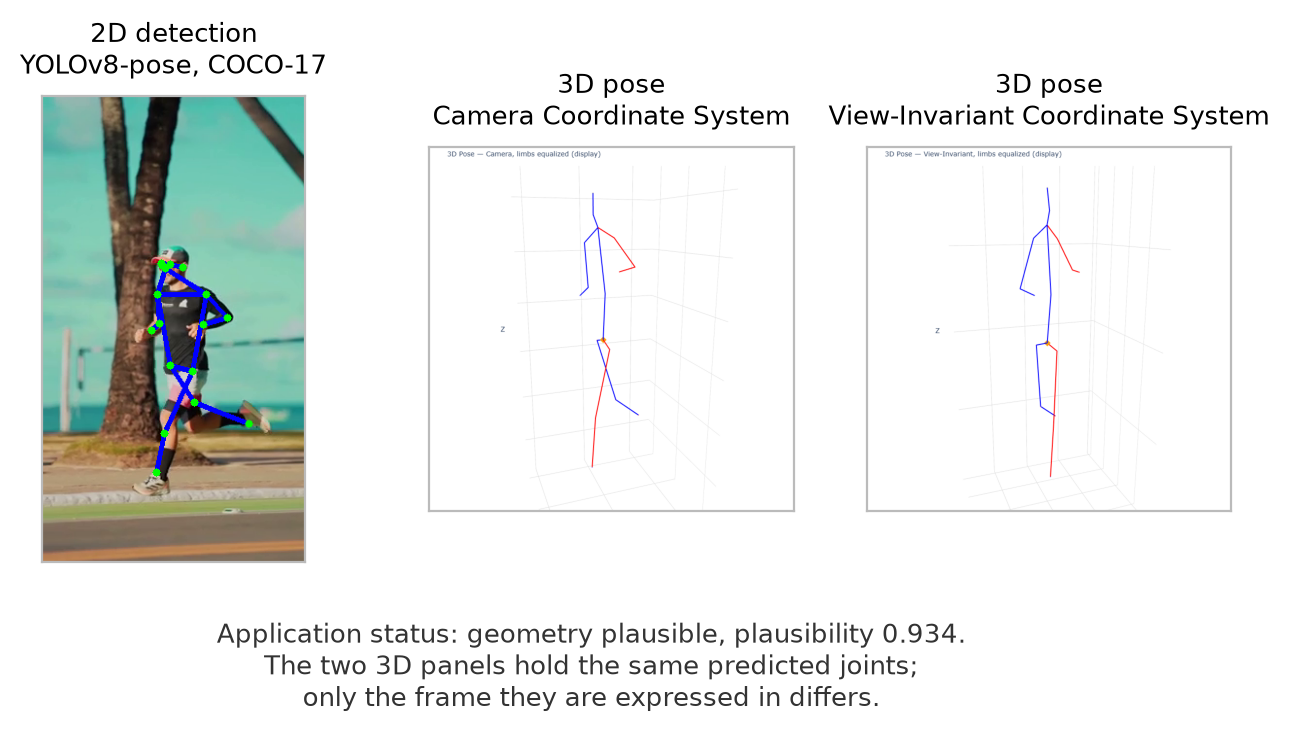
\includegraphics[width=\textwidth]{images/fig_app.png}
\caption[What the demonstration application returns]{What the demonstration application returns for a single frame, produced by calling the same entry point the evaluation uses. The reported numbers and the demonstrated behaviour therefore cannot diverge.}
\label{fig:app}
\end{figure}


\begin{figure}[H]
\centering
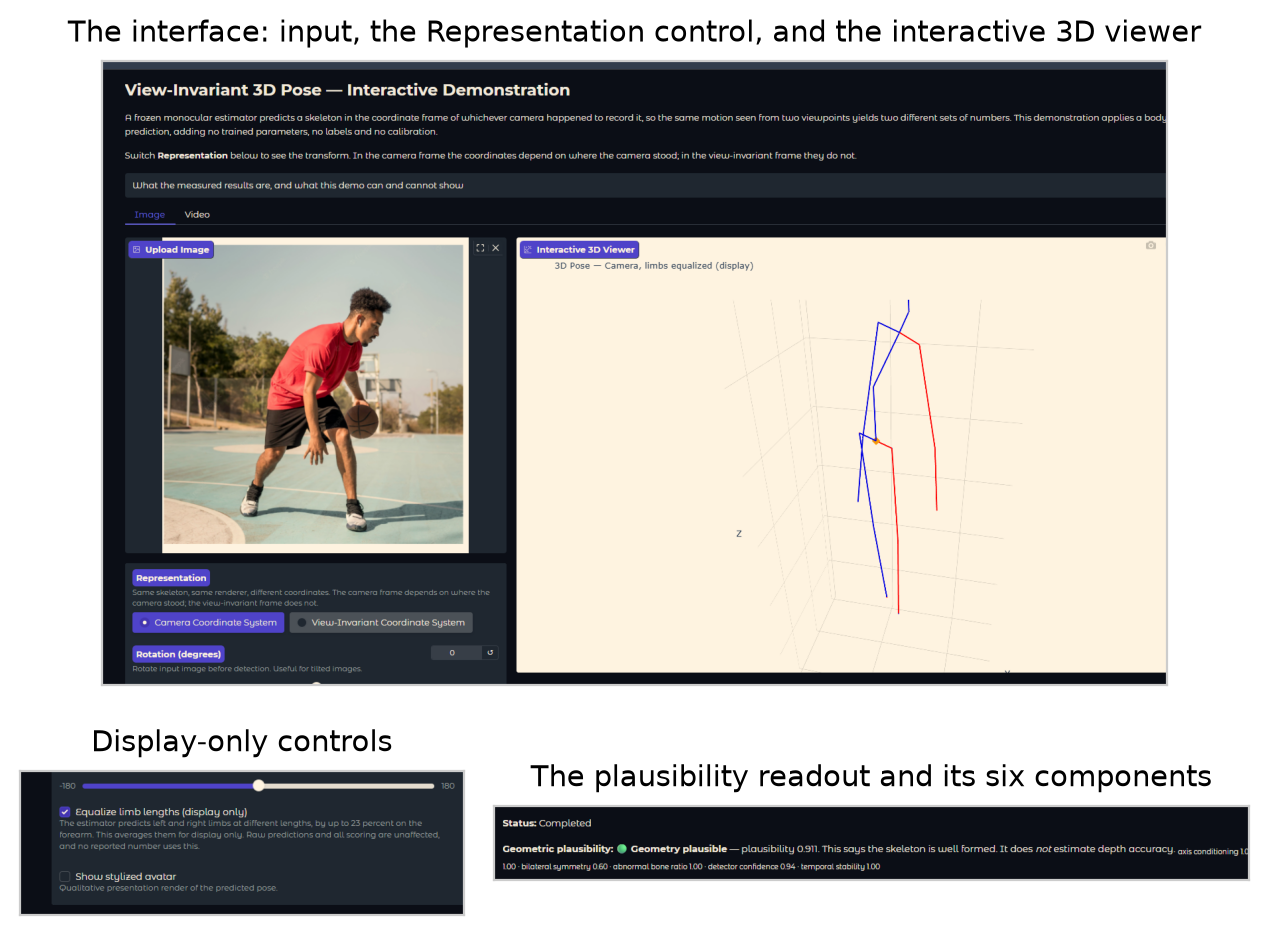
\includegraphics[width=\textwidth]{images/fig_interface.png}
\caption[The demonstration interface]{The demonstration interface. The Representation control switches between the camera frame and the body-fixed frame.}
\label{fig:interface}
\end{figure}


Figures~\ref{fig:app} and~\ref{fig:interface} show the demonstration application and its interface, both of which call the same entry point the evaluation uses, so what is shown and what is measured cannot diverge. The interface displays the plausibility readout with its own caution: it is a degeneracy gate, not a confidence score, and this report falsifies it as a predictor of accuracy. The reproduced MotionAGFormer-XS baseline matches the published benchmark results \cite{motionagformer} to within 0.05~mm, achieving an MPJPE of 45.149~mm compared with the reported 45.1~mm and a P-MPJPE of 36.892~mm compared with the reported 36.9~mm. Because the original publication reports values to only one decimal place, a more precise comparison is possible only against the official evaluation code provided by the backbone authors, which our implementation reproduces to three decimal places.

This verification establishes that the experimental pipeline faithfully reproduces the reference implementation. Consequently, the negative findings reported throughout this chapter can be attributed to the evaluated hypotheses rather than to implementation errors in the underlying pose estimation system.

\section{The Central Claim: Cross-View Comparability}
\label{sec:h36mcv}

\begin{figure}[H]
\centering
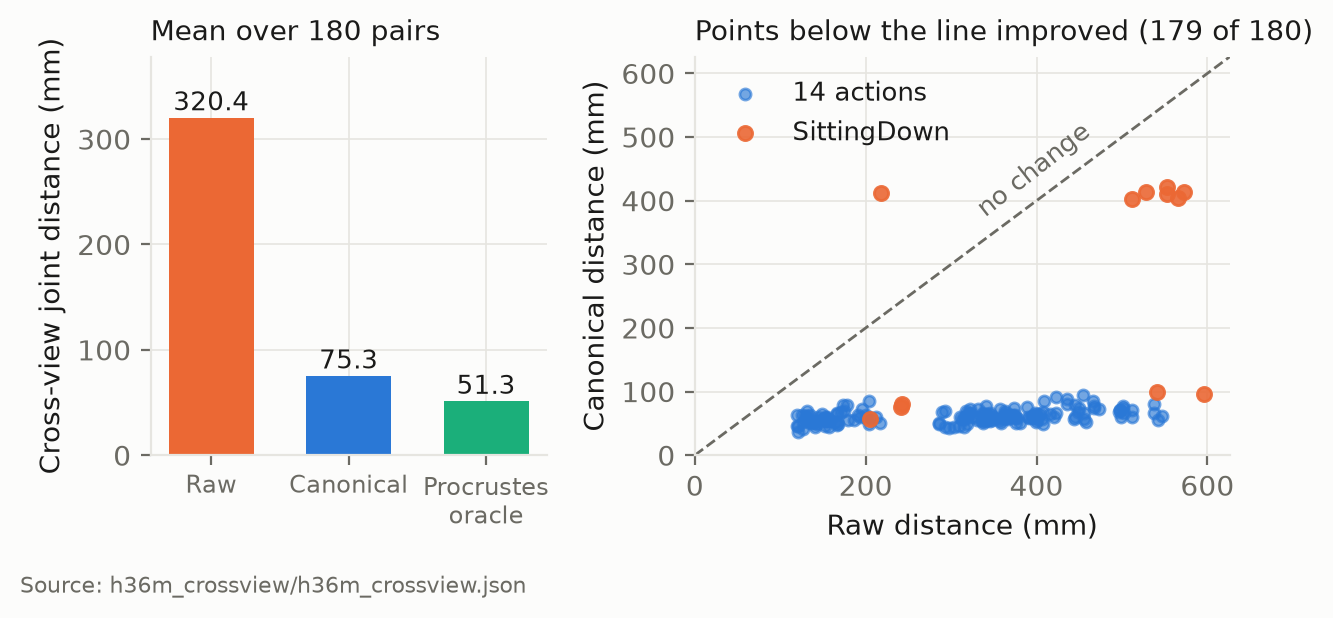
\includegraphics[width=\textwidth]{images/fig_h36m_distances.png}
\caption[Cross-view distance per camera pair, before and after]{The headline result as a distribution rather than a mean. Each point is one of the 180 held-out camera pairs, before and after canonicalization. The single pair that does not improve is visible, and is reported rather than trimmed.}
\label{fig:distances}
\end{figure}


% [H] deliberately: at its two-row height this figure fills a page of its own, so
% floating it only moves it away from the text that discusses it.
\begin{figure}[H]
\centering
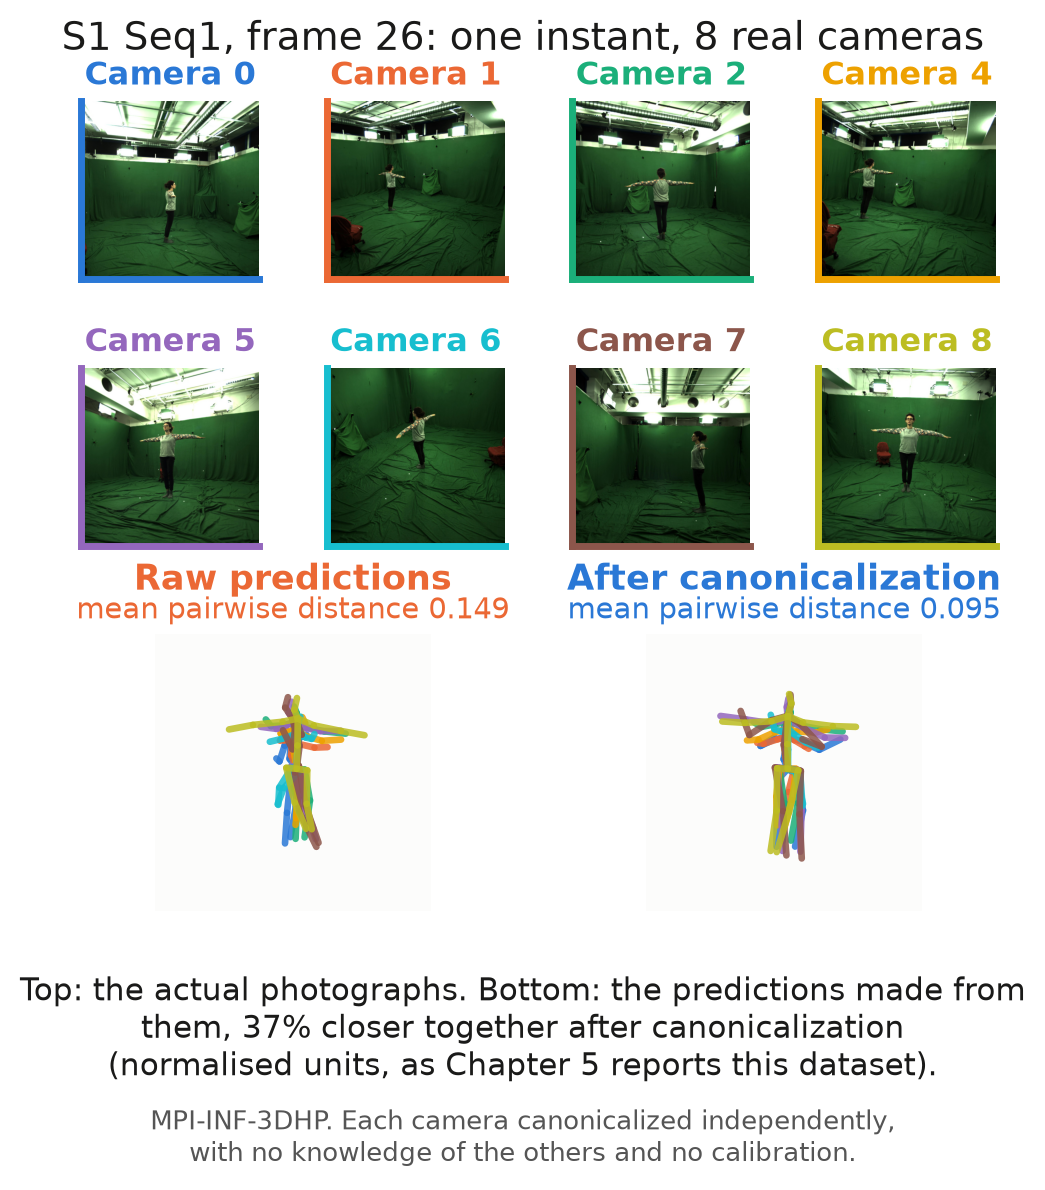
\includegraphics[width=\textwidth]{images/fig_realview.png}
\caption[The effect on eight real cameras]{What the method does, on photographs rather than stick figures. One instant of MPI-INF-3DHP seen by all eight synchronized cameras. Below left, the eight predictions in their own camera frames: the same pose eight times, and they do not overlap. Below right, the same eight after canonicalization, each camera processed independently, in ignorance of the others and without calibration. Mean pairwise distance falls from 0.149 to 0.095 in the normalised units the cache stores, a reduction of 36.6 percent.}
\label{fig:realview}
\end{figure}

Figure~\ref{fig:realview} is a single frame, and it illustrates rather than measures. Table \ref{tab:crossview} is the answer to the question a reader asks first---how does the proposed output compare to the base output. Accuracy is identical by construction: the estimator is frozen and canonicalization adds zero parameters. What changes is agreement between cameras.

\begin{table}[H]
\centering
\caption[Base output versus proposed output]{Base output vs proposed output on Human3.6M (MotionAGFormer-XS, 180 held-out camera pairs).}
\label{tab:crossview}
\small
\begin{tabular}{>{\raggedright\arraybackslash}p{4.9cm}cc>{\raggedright\arraybackslash}p{3.5cm}}
\toprule
 & \textbf{Base} & \textbf{Proposed} & \textbf{Change} \\
\midrule
MPJPE vs ground truth & 45.149 mm & 45.149 mm & identical \\
Cross-view distance, 13 non-constructor joints & 372.7 mm & 93.4 mm & $-72.2\%$ \\
Cross-view distance, all 17 joints & 320.4 mm & 75.3 mm & $-74.1\%$ \\
Per-frame Procrustes oracle & --- & 56.2 mm & 87.0\% of gap closed \\
Pairs improved (13-joint) & --- & 179 / 180 & --- \\
Added trained parameters & 0 & 0 & none \\
Added cost per frame & --- & 402 FLOPs & --- \\
Requirements & detector + lifter & unchanged & no training, labels or calibration \\
\bottomrule
\end{tabular}
\end{table}

The headline result excludes the four joints used to construct the reference frame, because those joints are partially constrained by the construction itself (the thorax canonicalizes at 22.1~mm against 197.5~mm for articulated joints). Including them would therefore overstate the improvement. Under this evaluation protocol, canonicalization reduces the mean cross-view distance by 72.2 percent, with a cluster-bootstrap confidence interval of $[+67.9, +75.5]$ computed over the thirty subject--action clusters. Figure~\ref{fig:distances} shows the same result as a distribution over the 180 pairs rather than as a mean, and Figure~\ref{fig:realview} shows the operation on eight real camera views of one instant.

The same algorithm was applied without modification to the second backbone, MotionBERT, where it improved cross-view distance by 75.8 percent across 180 of 180 evaluated camera pairs. One qualification should be stated rather than waited for. Although MotionAGFormer-XS was trained on Human3.6M, only the \emph{backbone} is in-domain; the \emph{method} itself was developed exclusively on MPI-INF-3DHP and applied here without further tuning.

\section{A Single-View Baseline, and It Wins}
\label{sec:template}

\begin{figure}[H]
\centering
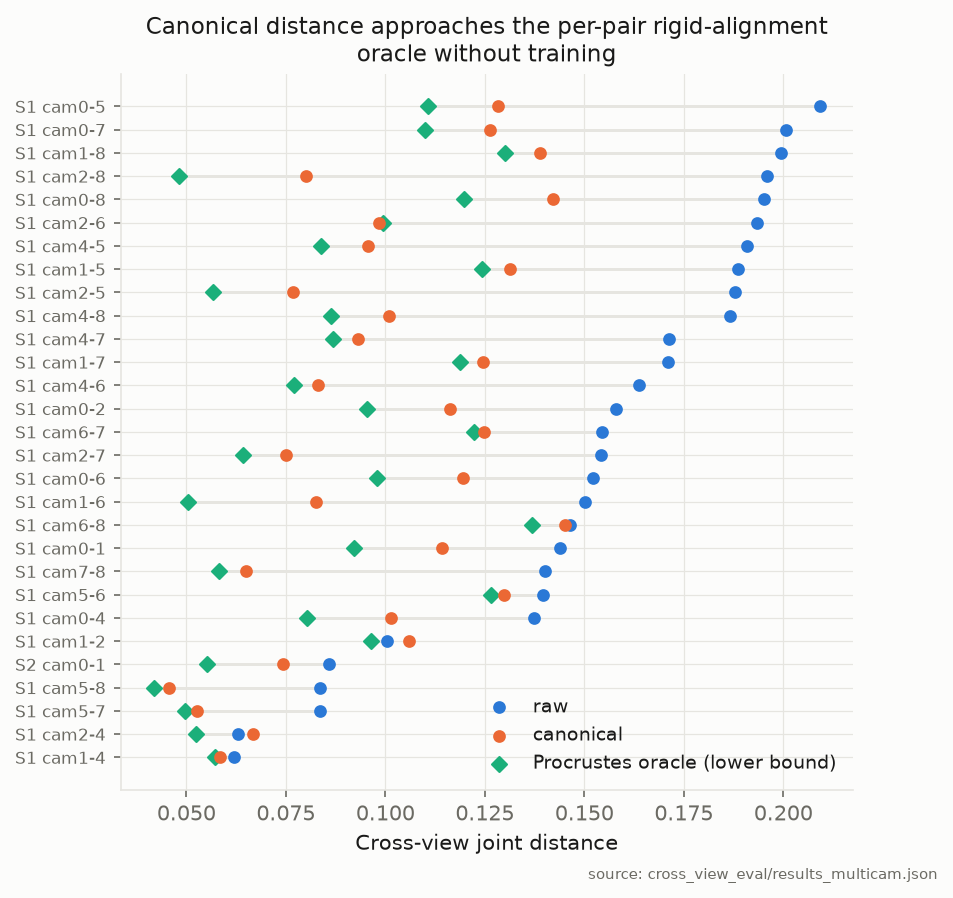
\includegraphics[width=\textwidth]{images/fig_oracle.png}
\caption[The method against the Procrustes floor]{Where the method sits against its floor. The per-frame Procrustes oracle is allowed to see both views and is therefore unreachable by any single-view method; it bounds how much of the remaining disagreement is removable by rotation at all.}
\label{fig:oracle}
\end{figure}

Kabsch-aligning \cite{kabsch} each predicted pose onto one fixed reference skeleton is training-free, label-free, calibration-free and single-view---it meets every requirement this framework claims as its profile, and it is what V-VIPE uses as preprocessing. It was pre-registered before it was run, including all three readings of the outcome. Figure~\ref{fig:oracle} places the anatomical frame against the per-frame Procrustes oracle, which is allowed both views and therefore bounds how much of the remaining disagreement is removable by rotation at all.

\begin{table}[H]
\centering
\caption[The pre-registered baseline comparison]{The pre-registered baseline comparison (13 non-constructor joints, XS).}
\label{tab:template}
\begin{tabular}{lcc}
\toprule
 & \textbf{Anatomical frame} & \textbf{Kabsch-to-template} \\
\midrule
Cross-view distance & 93.4 mm & \textbf{57.5 mm} \\
Camera pairs where it wins & 0 / 180 & \textbf{180 / 180} \\
\bottomrule
\end{tabular}
\end{table}

Table~\ref{tab:template} reports the outcome. The baseline wins on both backbones, all fifteen actions, under three unrelated templates and every centring tested, with the paired-difference interval excluding zero. This result is reported in the abstract, here, in the limitations, and in the conclusion. The method is kept because the baseline \emph{cannot run the experiment this report is about}: Kabsch alignment has no anatomical axis, so there is no axis to hold fixed and vary, and the question of what governs frame consistency cannot be posed inside it. As a way of reducing cross-view distance on this data, the simpler method is better, and we say so plainly. Section~\ref{sec:closing} returns to this with an experimental answer rather than a rhetorical one.

\section{A Second Backbone}
\label{sec:backbone2}

The framework consumes a seventeen-by-three array and nothing else, so
independence from the estimator is structural. It is not, on that argument
alone, empirical. We test it by replacing the backbone and changing nothing
else: MotionBERT, roughly nineteen times larger than MotionAGFormer-XS, with the
canonicalization code, the protocol, the joint sets and the statistical
treatment all unmodified. Table~\ref{tab:backbone} reports the outcome.

\begin{table}[H]
\centering
\caption[The central result under both backbones]{The central result under both backbones. Same code, same protocol, same 180 held-out camera pairs.}
\label{tab:backbone}
\begin{tabular}{lcc}
\toprule
& MotionAGFormer-XS & MotionBERT \\
\midrule
Raw cross-view distance, 13 joints & 372.7 mm & 368.0 mm \\
After canonicalization & 93.4 mm & 74.8 mm \\
Improvement & $+72.2\%$ & $+75.8\%$ \\
Pairs improved & 179 / 180 & 180 / 180 \\
Over all 17 joints & $+74.1\%$ & $+77.5\%$ \\
Added parameters & 0 & 0 \\
\bottomrule
\end{tabular}
\end{table}

\noindent The improvement is slightly larger on the stronger backbone, which is
the expected direction: canonicalization removes the camera rotation exactly, so
what remains is the estimator's own error, and a better estimator leaves less of
it. \textbf{Two backbones is replication, not universality.} Every claim in this
report that depends on the estimator is stated for $n = 2$, and the one signal
that behaved differently on a third architecture --- the reliability score, whose
correlation with error changed sign on a plain multi-layer perceptron --- is
reported as falsified partly because of it.

\section{The Axis-Length Boundary}
\label{sec:axisboundary}

\begin{figure}[H]
\centering
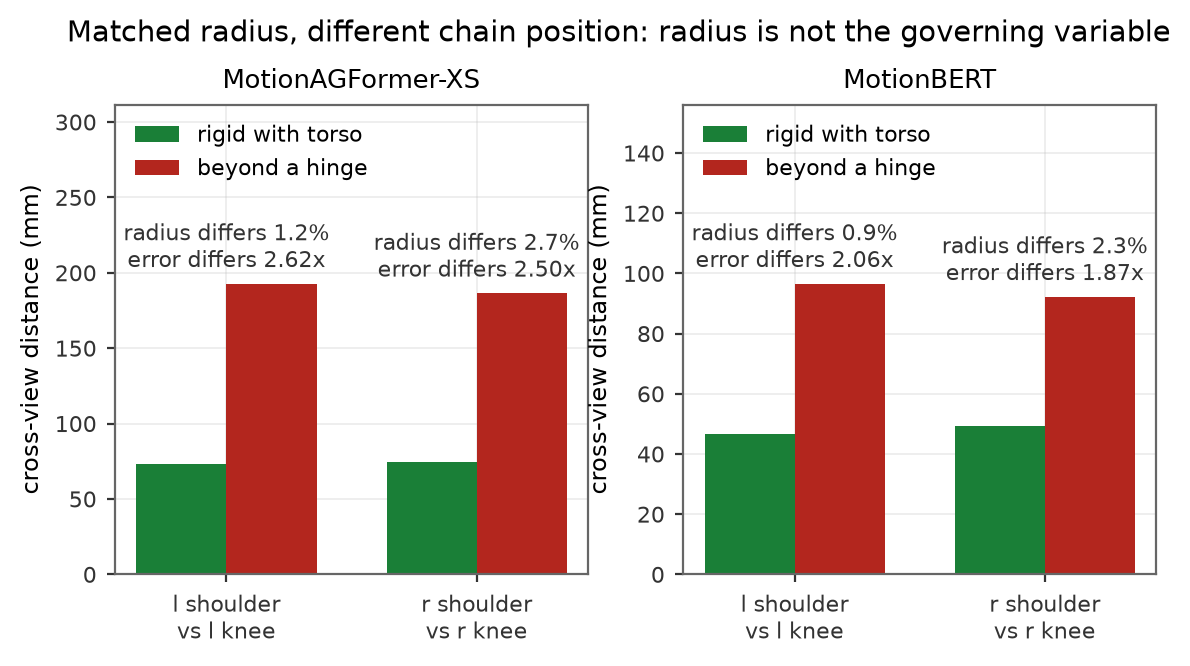
\includegraphics[width=0.9\textwidth]{images/fig_matched_radius.png}
\caption[Articulation, not radius, governs per-joint disagreement]{Matched-radius joint pairs: joints rigid with the torso against joints beyond a hinge, at comparable mean radius.}
\label{fig:matchedradius}
\end{figure}

\begin{figure}[H]
\centering
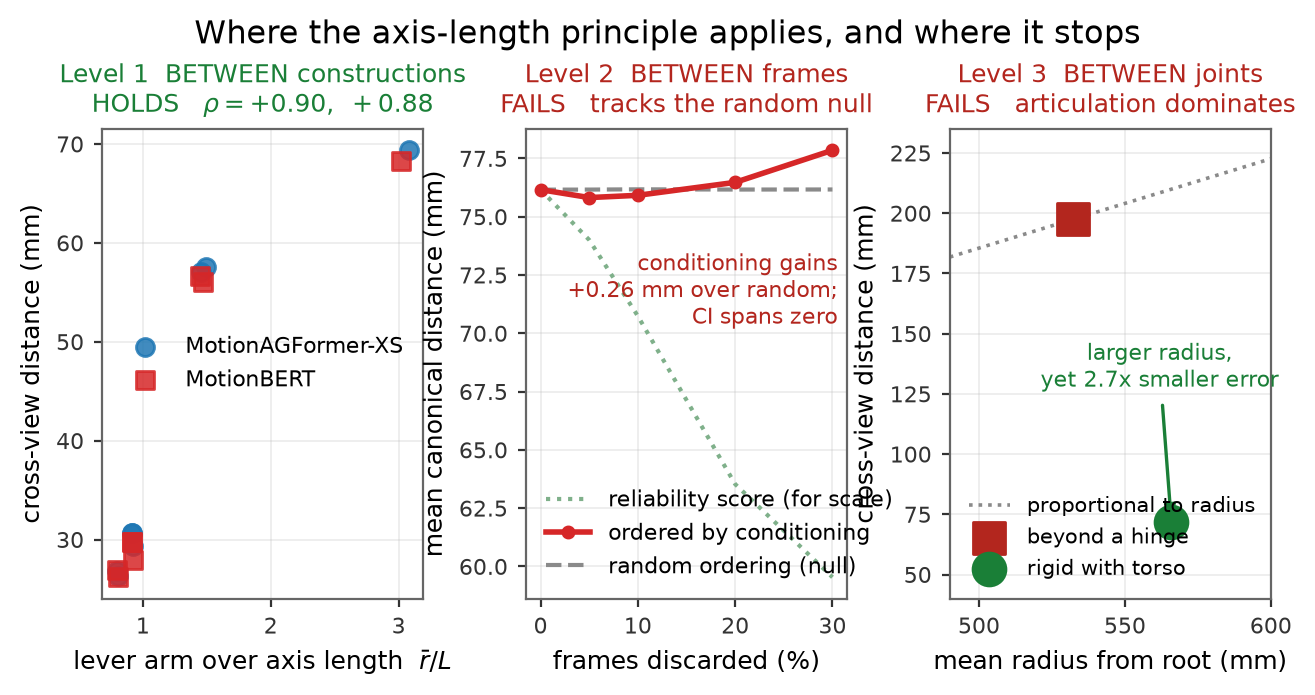
\includegraphics[width=\textwidth]{images/fig_three_levels.png}
\caption[The three levels of the axis-length boundary]{The three levels at which the axis-length principle was tested, and the two at which it fails.}
\label{fig:threelevels}
\end{figure}


The derived law of Equation~\ref{eq:theta} is tested at three levels, each pre-registered, and Figure~\ref{fig:threelevels} summarizes the three together with the two at which it fails.

\paragraph{Between constructions.} The principle holds. Holding the joint set, the scored set and the constructor count identical and replacing the hip axis with the longer shoulder axis improves the global frame on both backbones, by 5.2 and 4.4 percent, with intervals excluding zero.

\paragraph{Which frame within a construction to trust.} It fails. The per-limb multi-scale extension previously reported 55.1 percent; each limb frame is built from exactly the three joints it is then scored on, which removes the orientation being measured by construction. A per-segment Procrustes control confirms it, and the figure is demoted to exploratory.

\paragraph{Which joint will disagree.} It fails, and the reason is the finding. The radius model predicts per-joint disagreement from distance to the frame origin; its slope is 0.218 with $R^2 = 0.34$, far outside the pre-registered predicted band $[0.038, 0.073]$. The control explains it: joints rigid with the torso sit at a \emph{larger} mean radius than articulated joints and yet disagree by a factor of two and a half \emph{less}---the shoulder and knee agree to within 1--3 percent in radius and differ by roughly a factor of two in canonical distance. Articulation dominates; the frame-geometry model is the wrong model at this level. Figure~\ref{fig:matchedradius} shows the matched-radius pairs on which this control rests.

\section{Reliability: Falsified, and What It Is For}

The analytic reliability score was tested as an accuracy predictor five ways: correlation near zero across simultaneous cameras; view selection no better than chance; opposite signs on the two backbones; reliability-weighted fusion worse than an unweighted mean (92.6 vs 88.5~mm); and a pre-registered test-time-augmentation test failing all criteria (pooled $\rho = 0.10$, interval $[-0.59, 0.48]$). The common pattern is that geometric plausibility survives depth errors: a network wrong about depth can still produce a skeleton that looks anatomically perfect.

The same score, however, gates the quantity its own specification names---canonicalization quality. Dropping the worst thirty percent of frames by score reduces mean cross-view distance by 22 percent, against a random baseline that does not move it, and the triage survives a bone-deviation confound control on both backbones (gain at ten percent abstention 5.4~mm, interval $[+1.5, +9.3]$). This was a comparator in its pre-registration, not its subject, and is reported as exploratory.

\section{Retractions and Failed Pre-registrations}
\label{sec:h36m}

\begin{figure}[H]
\centering
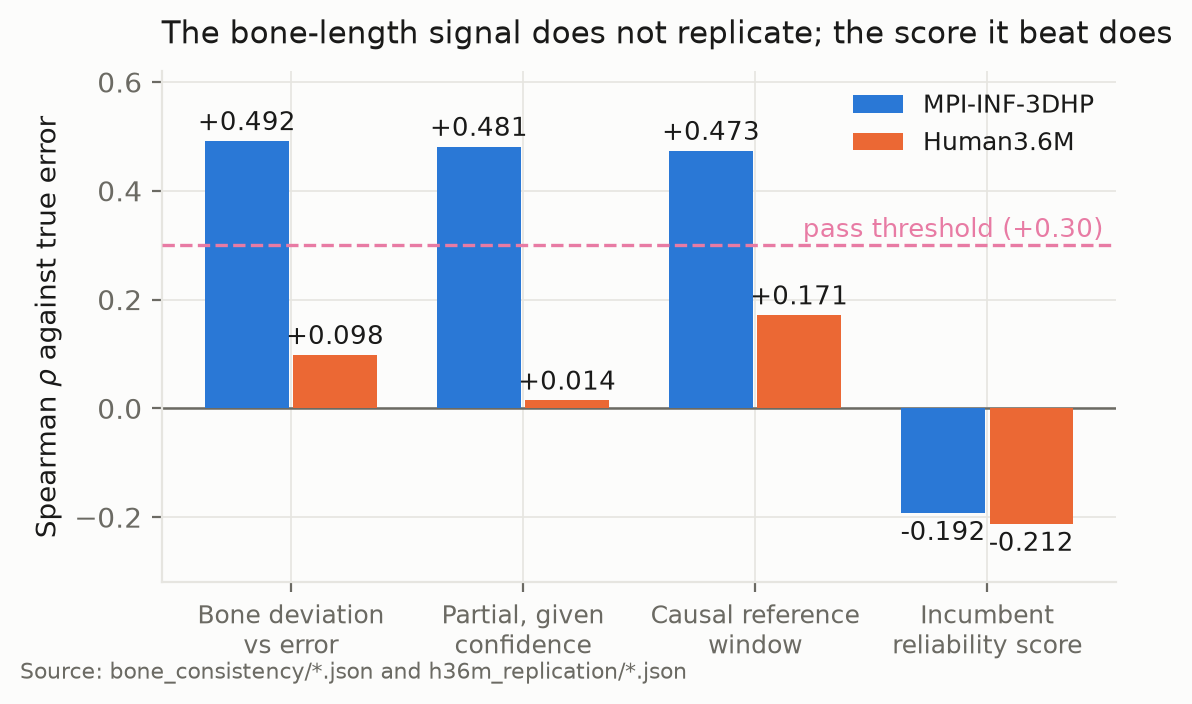
\includegraphics[width=0.9\textwidth]{images/fig_h36m_bone.png}
\caption[The retracted bone-length signal]{The retraction. A temporal bone-length signal that looked like a genuine error predictor on the first dataset does not survive on the second, and every pre-registered criterion fails there.}
\label{fig:bone}
\end{figure}

A temporal bone-length signal reached $\rho = +0.492$ on MPI-INF-3DHP and fell to $+0.098$ on Human3.6M, failing every criterion (Figure~\ref{fig:bone}); it is retracted, and the narrower condition under which it holds is stated in the full report. Two post-freeze pre-registrations also failed. Corrupting the eight distal joints of the predicted pose leaves the anatomical frame exactly flat at 53.45~mm at every severity (it never reads them) while the Kabsch baseline degrades from 43.3 to 92.3~mm---but the crossover the pre-registration required at $\sigma \le 80$~mm on both backbones fired on MotionBERT at 40~mm and on MotionAGFormer only at 160~mm, so the regime was not established at the committed severity. And scaling the template's limbs to child-like proportions moves the baseline by 0.12~mm (0.2 percent): the baseline needs no matching template.

\section{Fusion}
\label{sec:fusion}

In the shared frame, with eight views a median improves the aggregate while an unweighted mean does not, and the median's advantage grows as the number of views falls, as the breakdown analysis predicts. But the gain is not uniform across actions---nine of fifteen actions improve and six worsen---so the aggregate conceals a bimodal distribution, and the mean across actions is negative.

\section{Post-Freeze Addendum: Where the Two Alignments Fail, and a Routing Rule}
\label{sec:addendum}

Two pre-registered experiments (7 August 2026, commits preceding results in the repository history) complete the map of Section 5.3. The distal-corruption experiment showed the anatomical frame is immune to corruption of joints it never reads. Its mirror, corrupting the frame's own support joints \{1 r-hip, 4 l-hip, 8 thorax\}, shows the frame collapses while the 17-joint Kabsch fit degrades gracefully (Table \ref{tab:anchor}).

\begin{table}[H]
\centering
\caption[Anchor-joint corruption]{Anchor-joint corruption: the frame's failure is concentrated in its four-joint support (cross-view distance, mm).}
\label{tab:anchor}
\begin{tabular}{lcccc}
\toprule
$\sigma$ (mm) & XS anatomical & XS template & MB anatomical & MB template \\
\midrule
0 & 53.45 & 43.30 & 44.13 & 40.96 \\
20 & 71.95 & 43.70 & 64.57 & 41.38 \\
40 & 103.91 & 44.87 & 99.40 & 42.61 \\
80 & 215.66 & 49.15 & 217.81 & 47.15 \\
160 & 337.87 & 63.22 & 339.86 & 61.63 \\
\bottomrule
\end{tabular}
\end{table}

The failure supports are disjoint: distal corruption is invisible to the frame and visible to the template; anchor corruption is catastrophic for the frame and diluted in the 17-joint fit. A four-joint Kabsch control collapses with the frame, proving the effect is the joint support, not the anatomical construction.

This complementarity yields a decision rule. In deployment a detector reports per-joint confidence; the rule uses the anatomical frame iff the core joints $\{1, 4, 8\}$ are reliable (minimum confidence $\ge 0.7$) and the distal joints are not (minimum confidence $< 0.7$), else template Kabsch. \textbf{The weakness comes first, because it governs how the result should be read.} The corruption experiments inject noise with no confidence channel, so the rule's input is simulated as $c_j = \mathrm{clip}(1 - \sigma_j/80, 0, 1)$ where $\sigma_j$ is the noise applied to joint $j$. That signal is computed from the injected noise \emph{and from which joint set was corrupted}, so the rule is not inferring the regime: it is told the regime, and choosing the alignment that does not read the corrupted joints is then close to tautological. This is the same defect that Section~\ref{sec:axisboundary} demotes the multi-scale variant for, and by that standard the rule is exploratory rather than established. Evaluated over both corruption regimes and both backbones (Table \ref{tab:routing}), the routed distance attains the better single alignment's aggregate mean at 19 of 20 cells, trails it by 5.4~mm in the single transition cell (tolerance 7~mm, pre-registered, mean-level), and beats template-Kabsch alone by 38.8~mm (XS) and 47.3~mm (MB) at $\sigma = 160$~mm distal corruption, with bootstrap intervals excluding zero. At clean data the rule uses Kabsch---the better method there---and under anchor corruption it never routes into the collapsed arm. Three boundaries are stated with the result: the evaluation is of the conditional choice per corruption level (the confidence is constant within a level), not of per-frame decisions with noisy real confidence; the simulated signal is a noiseless encoding of the corruption, so the gain is an upper bound on a real confidence channel; and ``never worse'' holds for aggregate means, not pair by pair (in the transition cell the routed arm is worse than the better single alignment for every pair).

\begin{table}[H]
\centering
\caption[Confidence-gated routing against each single alignment]{Confidence-gated routing vs each single alignment (cross-view distance, mm).}
\label{tab:routing}
\begin{tabular}{llcccc}
\toprule
Regime & $\sigma$ (mm) & Route & Routed (XS) & t17 (XS) & Routed (MB) \\
\midrule
distal & 0 & t17 & 43.30 & 43.30 & 40.96 \\
distal & 40 & anat & 53.45 & 48.05 & \textbf{44.13} \\
distal & 80 & anat & \textbf{53.45} & 59.83 & \textbf{44.13} \\
distal & 160 & anat & \textbf{53.45} & 92.29 & \textbf{44.13} \\
anchor & 40 & t17 & 44.87 & 103.91 & 42.61 \\
anchor & 160 & t17 & 63.22 & 337.87 & 61.63 \\
\bottomrule
\end{tabular}
\end{table}

The honest boundaries are stated alongside the result: the confidence signal is simulated, not measured, and noiseless---an upper bound on a real confidence channel; the corruption is injected Gaussian noise rather than real occlusion; ``never worse'' is mean-level within a pre-registered 7~mm transition allowance on one dataset and two backbones; the 5.4~mm transition shortfall is a point estimate whose interval is not established (at the neighbouring severity the XS interval spans zero); and the threshold is fixed, not tuned. The rule does not make the anatomical frame win, and it does not beat the better single alignment either: a selector between two arms cannot exceed the better arm, and on MotionAGFormer-XS the routed column equals the better arm in nine of its ten cells and is 5.4~mm worse in the tenth. The 38--47~mm figure is the margin over \emph{template alignment alone}, not over the better arm. What the rule buys is the max operation, and only because it is told which arm to take. What it demonstrates, stated exactly, is that \emph{given} knowledge of which joints are corrupted, an alignment that ignores those joints can be selected profitably. It does not demonstrate that such knowledge is obtainable, and the next section establishes that on this pipeline it is not.

A fourteenth pre-registration (same date) closes the last avenue an examiner is likely to try: does the corruption matter end-to-end, through the real detection path? Re-running the real YOLOv8 detection on MPI-INF-3DHP S1/Seq1 cameras 0 and 1 (the clean re-lift reproduces the cached predictions to 0.00~mm) and displacing the 2D keypoints of the distal and core joint groups by up to 21 percent of the frame width---0.6 in the normalized input space at the wrist---changes the lifted 3D pose by at most 0.33~mm mean (per-joint worst case 0.77~mm), at every magnitude tested (Table \ref{tab:misdetect}). The frozen lifter absorbs 2D keypoint error entirely; the pipeline's failure surface is at the 3D alignment level. The same run measures the real confidence channel: mean per-keypoint confidence is 0.74 and 0.81 on the two cameras with \emph{every} frame below 0.9, so no threshold can separate frames on clean data. \textbf{This removes the routing rule's premise rather than scoping it.} The rule needs a detector-confidence gate; on clean data that channel carries no usable signal. And since 2D error does not propagate to 3D, detector failure cannot produce the 3D corruption regimes the rule routes between either. The real pipeline supplies neither the gate nor the regime, so the rule stands as a conditional result about a situation not yet shown to arise. The measured signal that does vary is the analytic reliability score, which is where a deployable gate would have to come from. Prediction P2 of this pre-registration, which required the channel to be \emph{saturated}, failed: the measurement is the opposite, and the amended criterion that passes was written after seeing it.

\begin{table}[H]
\centering
\caption[2D-input invariance of the frozen lifter]{2D-input invariance of the frozen lifter through the real detection path (MPI-INF-3DHP S1/Seq1; mean per-joint $|\Delta|$ vs clean lift, mm).}
\label{tab:misdetect}
\begin{tabular}{lcc}
\toprule
Condition & cam0 & cam1 \\
\midrule
distal, f=0.03 (87 px) & 0.06 & 0.06 \\
distal, f=0.10 (290 px) & 0.15 & 0.18 \\
distal, f=0.15 (434 px) & 0.21 & 0.25 \\
core, f=0.03 & 0.15 & 0.08 \\
core, f=0.10 & 0.26 & 0.23 \\
core, f=0.15 & 0.32 & 0.33 \\
\midrule
detector confidence (mean) & 0.74 & 0.81 \\
frames with confidence $< 0.9$ & 100\% & 100\% \\
\bottomrule
\end{tabular}
\end{table}


\section{Closing the Search: Three Further Pre-registrations}
\label{sec:closing}

Sections \ref{sec:template} and \ref{sec:addendum} leave one question open. The
baseline comparison was run against the default frame construction, and the
corruption regimes tested so far were bilaterally symmetric. Three further
pre-registrations, committed before their runs like the rest, close both gaps.
None of them produces a regime in which the anatomical frame is preferable, and
the third explains why the search should stop.

\subsection{Was the Comparison Run Against the Wrong Frame?}

The baseline comparison calls the default two-vector construction, with the hip
axis primary. But the confirmed level-one result of Section \ref{sec:axisboundary}
is that axis length governs the choice between constructions, and that the longer
shoulder axis makes the better frame. The headline comparison was therefore run
against a construction this report's own principle predicts is suboptimal, and
the best one had never been put against Kabsch. The fifteenth pre-registration
does that, for all five constructions the framework implements, scored on the
nine joints that are a constructor for none of them so that no construction is
flattered by joints its own frame pins. Table~\ref{tab:bestframe} reports every
construction against the baseline.

\begin{table}[H]
\centering
\small
\caption[Every frame construction against the baseline]{Every frame construction against Kabsch-to-template, scored on the nine joints no construction builds from. Gain is positive when the frame is closer than the template.}
\label{tab:bestframe}
\begin{tabular}{lcccc}
\toprule
& \multicolumn{2}{c}{MotionAGFormer-XS} & \multicolumn{2}{c}{MotionBERT} \\
\cmidrule(lr){2-3}\cmidrule(lr){4-5}
Construction & mm & gain vs template & mm & gain vs template \\
\midrule
Two-vector, hip primary (default) & 115.01 & $-49.17$ & 91.74 & $-27.32$ \\
Hip axis only & 114.46 & $-48.62$ & 91.01 & $-26.59$ \\
Shoulder axis only & 108.16 & $-42.32$ & \textbf{86.87} & $-22.45$ \\
Weighted multi-landmark & 109.67 & $-43.83$ & 93.43 & $-29.01$ \\
Spine principal direction (SVD) & \textbf{107.33} & $-41.49$ & 101.94 & $-37.52$ \\
\midrule
\textbf{Kabsch to fixed template} & \textbf{65.84} & --- & \textbf{64.42} & --- \\
\bottomrule
\end{tabular}
\end{table}

\noindent \textbf{No construction beats the baseline, on either backbone, with every
interval excluding zero.} The result is therefore not an artifact of frame choice.
What the experiment does establish is that the published comparison understated
the method: the best construction is 7.68~mm better than the default on
MotionAGFormer-XS and 4.87~mm better on MotionBERT, so the true gap is 41.49~mm
rather than the 49.17~mm a reader would infer from the default alone. Over all
seventeen joints the same ordering holds, with the shoulder-axis frame at
71.37~mm against 53.03~mm for the template.

One honest qualification: there is no single best construction. The spine
principal direction wins on MotionAGFormer at nine joints, the shoulder axis
wins everywhere else, and the spine variant is \emph{worse} than the default on
MotionBERT, at 101.94~mm against 91.74. This is consistent with the level-one
finding, which ranks constructions by axis length rather than crowning one.

\subsection{Asymmetric Corruption}

Both corruption regimes tested so far were bilaterally symmetric. Since Kabsch
fits a rotation, and a symmetric perturbation leaves the point cloud's principal
axes where they are, a one-sided corruption might rotate the fit where a
balanced one does not. The sixteenth pre-registration corrupts only the left
distal joints, leaving the four the frame reads untouched. Table~\ref{tab:asymmetric}
reports the result.

\begin{table}[H]
\centering
\small
\caption[Left-side-only distal corruption]{Left-side-only distal corruption. The anatomical frame is flat by construction, since it reads none of the corrupted joints.}
\label{tab:asymmetric}
\begin{tabular}{lcccc}
\toprule
& \multicolumn{2}{c}{MotionAGFormer-XS} & \multicolumn{2}{c}{MotionBERT} \\
\cmidrule(lr){2-3}\cmidrule(lr){4-5}
$\sigma$ (mm) & anatomical & template & anatomical & template \\
\midrule
0 & 53.45 & \textbf{43.30} & 44.13 & \textbf{40.96} \\
40 & 53.45 & \textbf{45.72} & 44.13 & 43.50 \\
80 & 53.45 & 51.71 & \textbf{44.13} & 49.74 \\
160 & \textbf{53.45} & 70.68 & \textbf{44.13} & 69.43 \\
\bottomrule
\end{tabular}
\end{table}

\noindent The crossover arrives at 80~mm on MotionBERT and not until 160~mm on
MotionAGFormer-XS, a severity the pre-registration ruled out in advance. One
backbone is not two, which is the rule by which the conditioning index and the
tenth pre-registration were both rejected, so this fails on the same terms.

\subsection{Laterality, With the Confound Removed}

The comparison above is confounded: the one-sided set has four joints against the
earlier bilateral set's eight, so laterality and joint count moved together. The
seventeenth pre-registration holds the count and the anatomical types fixed --- one
knee, one foot, one elbow, one wrist in both arms --- and varies only which side
they sit on. Table~\ref{tab:laterality} reports it.

\begin{table}[H]
\centering
\small
\caption[Laterality at matched joint count]{Laterality at matched joint count. Positive would mean one-sided corruption damages the template alignment more, which is what was predicted.}
\label{tab:laterality}
\begin{tabular}{lccc}
\toprule
$\sigma$ (mm) & one-sided (mm) & balanced (mm) & one-sided $-$ balanced \\
\midrule
\multicolumn{4}{l}{\emph{MotionAGFormer-XS}} \\
80 & 51.71 & 52.23 & $-0.52$ \: $[-0.66, -0.38]$ \\
160 & 70.68 & 72.21 & $-1.53$ \: $[-1.86, -1.17]$ \\
\multicolumn{4}{l}{\emph{MotionBERT}} \\
80 & 49.74 & 50.27 & $-0.53$ \: $[-0.68, -0.37]$ \\
160 & 69.43 & 70.94 & $-1.51$ \: $[-1.82, -1.19]$ \\
\bottomrule
\end{tabular}
\end{table}

\noindent \textbf{The sign is negative wherever the interval excludes zero, on both
backbones. One-sided corruption damages the template alignment \emph{less}, not
more: the hypothesis is refuted rather than merely unsupported.} The two
backbones agree to two decimal places, $-0.52$ against $-0.53$ and $-1.53$
against $-1.51$, so this is a small effect measured precisely rather than a
marginal one read hopefully.

The mechanism accounts for the whole family. A rigid fit can absorb part of a
one-sided displacement by rotating toward it; a balanced displacement offers the
rotation nothing. Damage at $\sigma = 160$~mm orders accordingly: eight bilateral
joints cost the template 92.29~mm, four balanced joints 72.21~mm, four one-sided
joints 70.68~mm.

\subsection{Why the Search Stops Here}

\textbf{Laterality moves the template alignment by at most 1.53~mm, and in the
wrong direction.} On the same scored joints at clean data, the frame trails the baseline
53.45~mm to 43.30~mm on MotionAGFormer-XS and 44.13~mm to 40.96~mm on
MotionBERT, so the lever is several times smaller than the deficit on the
backbone where the crossover failed --- and its sign is backwards everywhere the
interval excludes zero, which settles the matter regardless of magnitude. The method-level gap on
the headline joint sets, 35.9 to 41.5~mm depending on the set, is larger still.
That is a quantitative reason to stop rather than another qualitative failure,
and it is worth more than the searches that preceded it: had the sign and the
effect size been measured first, several of those experiments would not have
been run.

The frame does win under severe distal corruption, at 160~mm on both backbones
and at 40~mm on MotionBERT. What no regime produced is a crossover at a severity
committed to in advance, on both backbones. Every pre-registered search has now
looked --- the per-action breakdown, distal corruption, template proportion
mismatch, every frame construction, one-sided corruption, and the laterality
control --- and the sentence that no pose regime favours this construction is
backed by all of them.

\newpage
\section{Comparative Context}
\label{sec:comparative}

Table~\ref{tab:comparative} places the numbers of this thesis beside the published
figures nearest to them. It is organised in three blocks, and the blocks are not
directly comparable: they use different datasets, different metrics and different
evaluation protocols, so no ranking across blocks is implied and none should be read
into the ordering of the rows. Table~\ref{tab:requirements} answers the separate
question of what each approach requires at deployment time.

Within Block C the comparison is controlled, and it is the one that matters here: the
same predictions, the same 180 held-out pairs and the same scored joints, differing only
in the alignment applied. The oracle row is included because it bounds what any rotation
can remove; it sees both views and is therefore not a method.

{\fontsize{9}{11}\selectfont
\setlength{\tabcolsep}{4pt}
\begin{longtable}{>{\raggedright\arraybackslash}p{4.3cm}>{\raggedright\arraybackslash}p{2.0cm}>{\raggedright\arraybackslash}p{3.4cm}>{\raggedright\arraybackslash}p{4.9cm}}
\caption[Comparative context]{Comparative context. The three blocks are not directly comparable: they use different datasets, metrics and evaluation protocols. No ranking across blocks is implied.}\label{tab:comparative}\\
\hline
\textbf{Method} & \textbf{Result} & \textbf{Metric} & \textbf{Dataset and protocol} \\
\hline
\endfirsthead
\multicolumn{4}{l}{\textit{Table \thetable\ (continued)}}\\
\hline
\textbf{Method} & \textbf{Result} & \textbf{Metric} & \textbf{Dataset and protocol} \\
\hline
\endhead
\multicolumn{4}{l}{\textbf{Block A: published prior work, as reported by its authors}} \\
3DPCNet, learned module \cite{3dpcnet} & 3.58$^\circ$ & Rotation error against a ground-truth canonical pose & MM-Fi \cite{mmfi}; the authors' own Table 1 \\
3DPCNet's anatomical baseline \cite{3dpcnet} & 20.6$^\circ$ & Rotation error against a ground-truth canonical pose & MM-Fi \cite{mmfi}; the authors' own Table 1 \\
\hline
\multicolumn{4}{l}{\textbf{Block B: reproduced in this thesis}} \\
MotionAGFormer-XS \cite{motionagformer} & 45.149~mm (published: 45.1) & MPJPE against ground truth & Human3.6M S9 and S11, action-balanced, twenty-seven-frame clips \\
\hline
\multicolumn{4}{l}{\textbf{Block C: measured in this thesis}} \\
No alignment (raw prediction) & 372.7~mm & Cross-view joint distance & Human3.6M, 180 held-out pairs, thirteen non-constructor joints \\
Anatomical body frame (this work) & 93.4~mm & Cross-view joint distance & As above \\
Kabsch-to-template \cite{kabsch} & \textbf{57.5~mm} & Cross-view joint distance & As above \\
Per-frame Procrustes oracle & 56.2~mm & Cross-view joint distance & As above; sees both views, so unreachable by any single-view method \\
\hline
\end{longtable}}

% ========================== CHAPTER 6 ================================
\chapter{DISCUSSION, CONCLUSION AND FUTURE WORK}
\label{ch:conclusion}

\section{Discussion}

Four weaknesses are stated rather than defended away. First, the core mechanism is a coordinate transform that predates this thesis by decades; the defence is the requirement profile and the boundary measurement, not the geometry. Second, the headline metric measures agreement, not correctness: two predictions wrong in the same way agree perfectly, and the oracle floor and the retained correlation with ground-truth error bound but do not eliminate this. Third, no downstream task succeeds---the retrieval experiment is negative---so the thesis improves a metric and never shows the metric buys anything; this is the honest ceiling on the work's significance. Fourth, two datasets, both laboratory multi-camera rigs, and two backbones is n = 2.

Against that, the negative results are real science: more than half the pre-registered experiments failed their own criteria, the failures are reported in the same detail as the successes, one competing method is reported as beating the proposed method, and 304 numbers trace to stored artifacts. That discipline is the thesis's actual contribution to a reader, and it is rarer at this level than any single result would be.

The post-freeze addendum sharpens the positioning without settling it. The two alignments fail on disjoint joint supports---a structural consequence of the frame reading four joints and Kabsch fitting seventeen, measured on both backbones, and the one new fact here that is not conditional on anything. What it does not yet buy is a method: the rule that would exploit it needs to know which joints are corrupted, and the same addendum shows that this pipeline does not supply that knowledge. The frame would be the right instrument when the core is reliable and the periphery is not; whether that situation is detectable, or arises at all outside injected noise, is unestablished.

\section{Conclusion}

This thesis asked what determines whether an anatomical reference frame is consistent across viewpoints, using a training-free canonicalization of a frozen estimator as the instrument. The answer, established by pre-registered experiments on two datasets and two backbones, is a boundary: axis length governs the choice between frame constructions and nothing finer; articulation, not radius, governs which joint disagrees; the reliability score fails as an accuracy predictor and works as a gate on canonicalization quality; and a simpler baseline beats the frame on the headline metric, which we report. The two alignments fail on disjoint joint supports, which is measured and unconditional. A confidence-gated rule exploiting that is never worse than the better single alignment within a pre-registered tolerance and 38--47~mm better than template alignment alone under severe distal corruption---but only given knowledge of which joints are corrupted, which the same set of experiments shows this pipeline does not provide. The map is a finding; the rule is exploratory.

Every pre-registered search for a pose regime in which the anatomical construction is preferable to the template baseline has failed, none finding one at a severity committed to in advance on both backbones. The last of them measured why: the largest effect available from manipulating corruption geometry is 1.5~mm, it points the wrong way, and the deficit it would need to overcome is several times larger on the same scored joints. That is the difference between a search abandoned and a search closed, and it is the more useful of the two outcomes.

\section{Future Work}

Proportional differences in body size were tested and produced no crossover: scaling the reference skeleton's limbs across a $\pm 40$ percent range moves the baseline by 0.12~mm. Genuinely asymmetric morphology---a subject whose left and right limbs differ---was not tested here and remains open. Real occlusion and real detector failure---rather than injected noise---would give the routing rule a defensible severity scale, and a deployment-grade confidence signal would replace the simulated one. A downstream task that consumes cross-view comparability, such as gait comparison across sessions, would show that the improved agreement buys something.

% ========================== REFERENCES ===============================
\renewcommand{\bibname}{REFERENCES}
% \newpage first: thebibliography opens with \chapter*, which starts a new page,
% so an entry added before it records the page BEFORE the heading. Starting the
% page here puts the entry, the anchor and the printed heading on one page.
\newpage
\phantomsection
\addcontentsline{toc}{chapter}{REFERENCES}
\begin{thebibliography}{99}

\bibitem{motionagformer} S. Mehraban, V. Adeli, and B. Taati, ``MotionAGFormer: Enhancing 3D Human Pose Estimation With a Transformer-GCNFormer Network,'' in \emph{Proc. IEEE/CVF Winter Conf. Applications of Computer Vision (WACV)}, 2024, pp. 6905--6915. doi: 10.1109/WACV57701.2024.00677.
\bibitem{motionbert} W. Zhu, X. Ma, Z. Liu, L. Liu, W. Wu, and Y. Wang, ``MotionBERT: A Unified Perspective on Learning Human Motion Representations,'' in \emph{Proc. IEEE/CVF Int. Conf. Computer Vision (ICCV)}, 2023, pp. 15039--15053. doi: 10.1109/ICCV51070.2023.01385.
\bibitem{h36m} C. Ionescu, D. Papava, V. Olaru, and C. Sminchisescu, ``Human3.6M: Large Scale Datasets and Predictive Methods for 3D Human Sensing in Natural Environments,'' \emph{IEEE Trans. Pattern Analysis and Machine Intelligence}, vol. 36, no. 7, pp. 1325--1339, 2014. doi: 10.1109/TPAMI.2013.248.
\bibitem{martinez} J. Martinez, R. Hossain, J. Romero, and J. J. Little, ``A Simple Yet Effective Baseline for 3D Human Pose Estimation,'' in \emph{Proc. IEEE Int. Conf. Computer Vision (ICCV)}, 2017, pp. 2659--2668. doi: 10.1109/ICCV.2017.288.
\bibitem{triad} H. D. Black, ``A Passive System for Determining the Attitude of a Satellite,'' \emph{AIAA Journal}, vol. 2, no. 7, pp. 1350--1351, 1964. doi: 10.2514/3.2555.
\bibitem{shuster} M. D. Shuster and S. D. Oh, ``Three-Axis Attitude Determination from Vector Observations,'' \emph{Journal of Guidance and Control}, vol. 4, no. 1, pp. 70--77, 1981. doi: 10.2514/3.19717.
\bibitem{dellacroce1999} U. Della Croce, A. Cappozzo, and D. C. Kerrigan, ``Pelvis and Lower Limb Anatomical Landmark Calibration Precision and Its Propagation to Bone Geometry and Joint Angles,'' \emph{Medical \& Biological Engineering \& Computing}, vol. 37, no. 2, pp. 155--161, 1999. doi: 10.1007/BF02513282.
\bibitem{dellacroce2005} U. Della Croce, A. Leardini, L. Chiari, and A. Cappozzo, ``Human Movement Analysis Using Stereophotogrammetry. Part 4: Assessment of Anatomical Landmark Misplacement and Its Effects on Joint Kinematics,'' \emph{Gait \& Posture}, vol. 21, no. 2, pp. 226--237, 2005. doi: 10.1016/j.gaitpost.2004.05.003.
\bibitem{videopose} D. Pavllo, C. Feichtenhofer, D. Grangier, and M. Auli, ``3D Human Pose Estimation in Video With Temporal Convolutions and Semi-Supervised Training,'' in \emph{Proc. IEEE/CVF Conf. Computer Vision and Pattern Recognition (CVPR)}, 2019, pp. 7745--7754. doi: 10.1109/CVPR.2019.00794.
\bibitem{3dpcnet} T. Ekanayake, C. \'{A}lvarez Casado, and M. Bordallo L\'{o}pez, ``3DPCNet: Pose Canonicalization for Robust Viewpoint-Invariant 3D Kinematic Analysis from Monocular RGB Cameras,'' in \emph{Proc. IEEE Int. Conf. Acoustics, Speech and Signal Processing (ICASSP)}, 2026, pp. 11007--11011. doi: 10.1109/ICASSP55912.2026.11464754.
\bibitem{3dpcnet2} Y. Liu, H. Jiang, H. Liu, R. Huang, and X. Ouyang, ``MoViD: View-Invariant 3D Human Pose Estimation via Motion-View Disentanglement,'' in \emph{Proc. ACM/IEEE Int. Conf. Embedded Artificial Intelligence and Sensing Systems (SenSys)}, 2026, pp. 1194--1207. doi: 10.1145/3774906.3802786.
\bibitem{smpl} M. Loper, N. Mahmood, J. Romero, G. Pons-Moll, and M. J. Black, ``SMPL: A Skinned Multi-Person Linear Model,'' \emph{ACM Trans. Graphics}, vol. 34, no. 6, art. 248, 2015. doi: 10.1145/2816795.2818013.
\bibitem{vvipe} M. Levy and A. Shrivastava, ``V-VIPE: Variational View Invariant Pose Embedding,'' in \emph{Proc. IEEE/CVF Conf. Computer Vision and Pattern Recognition Workshops (CVPRW)}, 2024, pp. 1633--1642. doi: 10.1109/CVPRW63382.2024.00170.
\bibitem{vihc} G. Wei, C. Lan, W. Zeng, and Z. Chen, ``View Invariant 3D Human Pose Estimation,'' \emph{IEEE Trans. Circuits and Systems for Video Technology}, vol. 30, no. 12, pp. 4601--4610, 2020. doi: 10.1109/TCSVT.2019.2928813.
\bibitem{kabsch} W. Kabsch, ``A Solution for the Best Rotation to Relate Two Sets of Vectors,'' \emph{Acta Crystallographica Section A}, vol. 32, no. 5, pp. 922--923, 1976. doi: 10.1107/S0567739476001873.
\bibitem{khanal} A. Khanal and J. Zhou, ``Severe Domain Shift in Skeleton-Based Action Recognition: A Study of Uncertainty Failure in Real-World Gym Environments,'' arXiv:2603.15574, 2026. (Preprint; not peer reviewed.)
\bibitem{yangpavone} H. Yang and M. Pavone, ``Object Pose Estimation With Statistical Guarantees: Conformal Keypoint Detection and Geometric Uncertainty Propagation,'' in \emph{Proc. IEEE/CVF Conf. Computer Vision and Pattern Recognition (CVPR)}, 2023, pp. 8947--8958. doi: 10.1109/CVPR52729.2023.00864.
\bibitem{wahba} G. Wahba, ``A Least Squares Estimate of Satellite Attitude,'' \emph{SIAM Review}, vol. 7, no. 3, p. 409, 1965. doi: 10.1137/1007077. (Problem 65--1; a one-page problem statement.)
\bibitem{cmanet} X. Li, M. Meng, Z. Wu, T. Chen, F. Yang, and D. Shen, ``Self-learning Canonical Space for Multi-view 3D Human Pose Estimation,'' arXiv:2403.12440, 2024. (Preprint; no peer-reviewed venue located.)
\bibitem{mmfi} J. Yang, H. Huang, Y. Zhou, X. Chen, Y. Xu, S. Yuan, H. Zou, C. X. Lu, and L. Xie, ``MM-Fi: Multi-Modal Non-Intrusive 4D Human Dataset for Versatile Wireless Sensing,'' in \emph{Advances in Neural Information Processing Systems 36 (NeurIPS), Datasets and Benchmarks Track}, 2023.
\bibitem{yolov8} G. Jocher, A. Chaurasia, and J. Qiu, ``Ultralytics YOLOv8,'' version 8.0.0, 2023. [Software]. Available: https://github.com/ultralytics/ultralytics
\bibitem{mpi} D. Mehta, H. Rhodin, D. Casas, P. Fua, O. Sotnychenko, W. Xu, and C. Theobalt, ``Monocular 3D Human Pose Estimation in the Wild Using Improved CNN Supervision,'' in \emph{Proc. Int. Conf. 3D Vision (3DV)}, 2017, pp. 506--516. doi: 10.1109/3DV.2017.00064.
\bibitem{hampel} F. R. Hampel, ``A General Qualitative Definition of Robustness,'' \emph{The Annals of Mathematical Statistics}, vol. 42, no. 6, pp. 1887--1896, 1971. doi: 10.1214/aoms/1177693054.
\bibitem{hourglass} A. Newell, K. Yang, and J. Deng, ``Stacked Hourglass Networks for Human Pose Estimation,'' in \emph{Computer Vision -- ECCV 2016}, LNCS vol. 9912, Springer, 2016, pp. 483--499. doi: 10.1007/978-3-319-46484-8\_29.
\end{thebibliography}

\appendix

\newpage

\chapter*{APPENDIX: COMPLETE RESULT TABLES}
\addcontentsline{toc}{chapter}{APPENDIX: COMPLETE RESULT TABLES}
\markboth{APPENDIX}{APPENDIX}
\setcounter{table}{0}
\renewcommand{\thetable}{A.\arabic{table}}

Every table in this appendix is generated from the stored JSON artifacts by
\texttt{python -m evaluation.make\_appendix\_tables} rather than typed by hand,
so it cannot drift from the figures the automated audit verifies. They are
reproduced here so a reader can trace any number in the body to its source
without leaving the document.

\begin{center}
{\fontsize{10}{12}\selectfont
\begin{longtable}{lrrrr}
\caption{Cross-view canonicalization on Human3.6M, by action.}\label{tab:appcvaction}\\
\hline
\textbf{Action} & \textbf{Pairs} & \textbf{Canonical (mm)} & \textbf{Improvement} & \textbf{Improved} \\
\hline
\endfirsthead
\multicolumn{5}{l}{\textit{(continued)}}\\
\hline
\textbf{Action} & \textbf{Pairs} & \textbf{Canonical (mm)} & \textbf{Improvement} & \textbf{Improved} \\
\hline
\endhead
\hline
\endfoot
Purchases & 12 & 61.9 & +81.4 & 12/12 \\
Sitting & 12 & 68.0 & +79.9 & 12/12 \\
Eating & 12 & 57.3 & +79.6 & 12/12 \\
WalkDog & 12 & 62.5 & +79.3 & 12/12 \\
Walking & 12 & 45.3 & +78.0 & 12/12 \\
Smoking & 12 & 59.6 & +77.6 & 12/12 \\
Phoning & 12 & 59.6 & +77.5 & 12/12 \\
WalkTogether & 12 & 53.2 & +77.1 & 12/12 \\
Waiting & 12 & 58.2 & +75.7 & 12/12 \\
Greeting & 12 & 61.4 & +75.0 & 12/12 \\
Discussion & 12 & 64.7 & +74.6 & 12/12 \\
Photo & 12 & 79.6 & +73.7 & 12/12 \\
Posing & 12 & 60.6 & +73.3 & 12/12 \\
Directions & 12 & 63.7 & +71.9 & 12/12 \\
SittingDown & 12 & 274.1 & +36.1 & 11/12 \\
\end{longtable}
}
\end{center}

\vspace{0.6cm}

\begin{center}
{\fontsize{10}{12}\selectfont
\begin{longtable}{llrrrrrr}
\caption{All 180 held-out Human3.6M camera pairs. Distances in millimetres.}\label{tab:apppairs}\\
\hline
\textbf{Subj} & \textbf{Action} & \textbf{Pair} & \textbf{N} & \textbf{Raw} & \textbf{Canon.} & \textbf{Oracle} & \textbf{Impr.} \\
\hline
\endfirsthead
\multicolumn{8}{l}{\textit{(continued)}}\\
\hline
\textbf{Subj} & \textbf{Action} & \textbf{Pair} & \textbf{N} & \textbf{Raw} & \textbf{Canon.} & \textbf{Oracle} & \textbf{Impr.} \\
\hline
\endhead
\hline
\endfoot
S11 & Directions & 01--02 & 154 & 341.1 & 76.6 & 56.1 & +77.5 \\
S11 & Directions & 01--03 & 154 & 128.7 & 61.3 & 50.6 & +52.3 \\
S11 & Directions & 01--04 & 154 & 373.5 & 74.0 & 57.8 & +80.2 \\
S11 & Directions & 02--03 & 154 & 364.2 & 61.0 & 49.8 & +83.3 \\
S11 & Directions & 02--04 & 154 & 156.3 & 54.5 & 40.7 & +65.1 \\
S11 & Directions & 03--04 & 154 & 345.2 & 66.6 & 55.3 & +80.7 \\
S11 & Discussion & 01--02 & 219 & 331.4 & 72.3 & 51.6 & +78.2 \\
S11 & Discussion & 01--03 & 219 & 134.7 & 62.6 & 47.5 & +53.5 \\
S11 & Discussion & 01--04 & 219 & 357.3 & 73.4 & 52.5 & +79.5 \\
S11 & Discussion & 02--03 & 219 & 347.5 & 55.6 & 45.7 & +84.0 \\
S11 & Discussion & 02--04 & 219 & 152.3 & 59.3 & 44.7 & +61.0 \\
S11 & Discussion & 03--04 & 219 & 319.4 & 66.2 & 52.6 & +79.3 \\
S11 & Eating & 01--02 & 219 & 449.9 & 74.6 & 62.1 & +83.4 \\
S11 & Eating & 01--03 & 219 & 171.0 & 67.6 & 54.8 & +60.5 \\
S11 & Eating & 01--04 & 219 & 498.2 & 70.9 & 63.9 & +85.8 \\
S11 & Eating & 02--03 & 219 & 458.5 & 52.6 & 46.6 & +88.5 \\
S11 & Eating & 02--04 & 219 & 193.3 & 60.2 & 52.0 & +68.9 \\
S11 & Eating & 03--04 & 219 & 445.0 & 60.6 & 55.4 & +86.4 \\
S11 & Greeting & 01--02 & 179 & 369.4 & 62.8 & 49.4 & +83.0 \\
S11 & Greeting & 01--03 & 179 & 152.0 & 53.6 & 44.6 & +64.7 \\
S11 & Greeting & 01--04 & 179 & 400.5 & 65.5 & 50.0 & +83.6 \\
S11 & Greeting & 02--03 & 179 & 391.6 & 59.2 & 48.4 & +84.9 \\
S11 & Greeting & 02--04 & 179 & 166.8 & 47.4 & 38.5 & +71.6 \\
S11 & Greeting & 03--04 & 179 & 362.6 & 63.7 & 51.7 & +82.4 \\
S11 & Phoning & 01--02 & 349 & 377.6 & 59.1 & 53.7 & +84.3 \\
S11 & Phoning & 01--03 & 349 & 148.7 & 64.2 & 55.6 & +56.8 \\
S11 & Phoning & 01--04 & 349 & 395.5 & 62.0 & 56.6 & +84.3 \\
S11 & Phoning & 02--03 & 349 & 406.8 & 56.4 & 50.7 & +86.1 \\
S11 & Phoning & 02--04 & 349 & 152.5 & 46.3 & 40.0 & +69.6 \\
S11 & Phoning & 03--04 & 349 & 374.6 & 59.0 & 53.4 & +84.2 \\
S11 & Posing & 01--02 & 141 & 343.4 & 65.5 & 51.6 & +80.9 \\
S11 & Posing & 01--03 & 141 & 130.8 & 62.1 & 46.3 & +52.6 \\
S11 & Posing & 01--04 & 141 & 375.2 & 62.4 & 48.5 & +83.4 \\
S11 & Posing & 02--03 & 141 & 357.9 & 50.9 & 44.8 & +85.8 \\
S11 & Posing & 02--04 & 141 & 149.6 & 56.7 & 41.9 & +62.1 \\
S11 & Posing & 03--04 & 141 & 338.0 & 61.6 & 47.2 & +81.8 \\
S11 & Purchases & 01--02 & 103 & 512.0 & 70.5 & 50.3 & +86.2 \\
S11 & Purchases & 01--03 & 103 & 200.7 & 58.9 & 43.5 & +70.7 \\
S11 & Purchases & 01--04 & 103 & 538.0 & 80.5 & 52.1 & +85.0 \\
S11 & Purchases & 02--03 & 103 & 546.8 & 61.2 & 44.9 & +88.8 \\
S11 & Purchases & 02--04 & 103 & 216.9 & 50.5 & 33.7 & +76.7 \\
S11 & Purchases & 03--04 & 103 & 496.8 & 67.8 & 49.6 & +86.4 \\
S11 & Sitting & 01--02 & 216 & 512.0 & 60.4 & 50.1 & +88.2 \\
S11 & Sitting & 01--03 & 216 & 191.4 & 62.5 & 48.5 & +67.3 \\
S11 & Sitting & 01--04 & 216 & 537.2 & 66.0 & 55.9 & +87.7 \\
S11 & Sitting & 02--03 & 216 & 542.3 & 55.8 & 46.6 & +89.7 \\
S11 & Sitting & 02--04 & 216 & 203.9 & 49.0 & 40.6 & +76.0 \\
S11 & Sitting & 03--04 & 216 & 498.6 & 59.6 & 51.8 & +88.0 \\
S11 & SittingDown & 01--02 & 200 & 527.8 & 413.6 & 79.0 & +21.6 \\
S11 & SittingDown & 01--03 & 200 & 241.1 & 76.1 & 70.8 & +68.4 \\
S11 & SittingDown & 01--04 & 200 & 552.4 & 410.4 & 73.3 & +25.7 \\
S11 & SittingDown & 02--03 & 200 & 565.4 & 404.7 & 62.6 & +28.4 \\
S11 & SittingDown & 02--04 & 200 & 205.6 & 57.6 & 53.8 & +72.0 \\
S11 & SittingDown & 03--04 & 200 & 511.6 & 403.0 & 69.8 & +21.2 \\
S11 & Smoking & 01--02 & 241 & 374.9 & 59.3 & 51.7 & +84.2 \\
S11 & Smoking & 01--03 & 241 & 154.2 & 60.4 & 52.9 & +60.8 \\
S11 & Smoking & 01--04 & 241 & 403.8 & 64.1 & 53.5 & +84.1 \\
S11 & Smoking & 02--03 & 241 & 399.6 & 58.9 & 51.6 & +85.3 \\
S11 & Smoking & 02--04 & 241 & 164.0 & 52.0 & 41.4 & +68.3 \\
S11 & Smoking & 03--04 & 241 & 373.0 & 62.7 & 55.8 & +83.2 \\
S11 & Photo & 01--02 & 198 & 423.1 & 90.9 & 75.8 & +78.5 \\
S11 & Photo & 01--03 & 198 & 178.1 & 79.0 & 65.3 & +55.6 \\
S11 & Photo & 01--04 & 198 & 454.2 & 94.0 & 77.4 & +79.3 \\
S11 & Photo & 02--03 & 198 & 445.6 & 78.3 & 61.4 & +82.4 \\
S11 & Photo & 02--04 & 198 & 195.5 & 72.7 & 56.2 & +62.8 \\
S11 & Photo & 03--04 & 198 & 408.8 & 85.1 & 70.4 & +79.2 \\
S11 & Waiting & 01--02 & 225 & 328.9 & 60.8 & 46.3 & +81.5 \\
S11 & Waiting & 01--03 & 225 & 126.8 & 52.8 & 43.4 & +58.4 \\
S11 & Waiting & 01--04 & 225 & 355.4 & 59.1 & 44.9 & +83.4 \\
S11 & Waiting & 02--03 & 225 & 345.2 & 53.9 & 44.0 & +84.4 \\
S11 & Waiting & 02--04 & 225 & 142.1 & 51.0 & 36.7 & +64.1 \\
S11 & Waiting & 03--04 & 225 & 324.8 & 59.6 & 45.8 & +81.6 \\
S11 & Walking & 01--02 & 162 & 297.0 & 43.1 & 36.2 & +85.5 \\
S11 & Walking & 01--03 & 162 & 126.3 & 41.2 & 34.2 & +67.4 \\
S11 & Walking & 01--04 & 162 & 318.6 & 49.7 & 42.7 & +84.4 \\
S11 & Walking & 02--03 & 162 & 315.0 & 44.7 & 39.2 & +85.8 \\
S11 & Walking & 02--04 & 162 & 121.1 & 36.1 & 31.2 & +70.2 \\
S11 & Walking & 03--04 & 162 & 292.7 & 44.8 & 38.9 & +84.7 \\
S11 & WalkDog & 01--02 & 144 & 467.1 & 74.7 & 48.6 & +84.0 \\
S11 & WalkDog & 01--03 & 144 & 206.8 & 58.0 & 46.4 & +71.9 \\
S11 & WalkDog & 01--04 & 144 & 502.4 & 66.9 & 48.1 & +86.7 \\
S11 & WalkDog & 02--03 & 144 & 497.5 & 71.8 & 50.7 & +85.6 \\
S11 & WalkDog & 02--04 & 144 & 211.5 & 59.7 & 45.0 & +71.8 \\
S11 & WalkDog & 03--04 & 144 & 448.9 & 68.1 & 53.7 & +84.8 \\
S11 & WalkTogether & 01--02 & 135 & 335.6 & 53.1 & 45.6 & +84.2 \\
S11 & WalkTogether & 01--03 & 135 & 142.7 & 49.5 & 43.2 & +65.3 \\
S11 & WalkTogether & 01--04 & 135 & 359.5 & 57.5 & 50.4 & +84.0 \\
S11 & WalkTogether & 02--03 & 135 & 357.1 & 54.1 & 48.5 & +84.8 \\
S11 & WalkTogether & 02--04 & 135 & 140.2 & 43.7 & 38.3 & +68.8 \\
S11 & WalkTogether & 03--04 & 135 & 330.6 & 54.6 & 48.9 & +83.5 \\
S9 & Directions & 01--02 & 268 & 289.1 & 67.4 & 52.6 & +76.7 \\
S9 & Directions & 01--03 & 268 & 119.4 & 63.4 & 47.3 & +46.9 \\
S9 & Directions & 01--04 & 268 & 310.4 & 60.4 & 55.0 & +80.5 \\
S9 & Directions & 02--03 & 268 & 313.1 & 57.5 & 51.9 & +81.6 \\
S9 & Directions & 02--04 & 268 & 134.4 & 51.3 & 37.9 & +61.8 \\
S9 & Directions & 03--04 & 268 & 292.7 & 70.1 & 57.7 & +76.0 \\
S9 & Discussion & 01--02 & 530 & 394.6 & 61.6 & 49.8 & +84.4 \\
S9 & Discussion & 01--03 & 530 & 166.5 & 64.1 & 48.7 & +61.5 \\
S9 & Discussion & 01--04 & 530 & 422.4 & 65.7 & 56.9 & +84.4 \\
S9 & Discussion & 02--03 & 530 & 416.3 & 64.4 & 54.3 & +84.5 \\
S9 & Discussion & 02--04 & 530 & 157.2 & 55.7 & 45.2 & +64.6 \\
S9 & Discussion & 03--04 & 530 & 388.8 & 75.0 & 59.9 & +80.7 \\
S9 & Eating & 01--02 & 268 & 380.3 & 50.5 & 39.3 & +86.7 \\
S9 & Eating & 01--03 & 268 & 145.6 & 55.5 & 38.3 & +61.9 \\
S9 & Eating & 01--04 & 268 & 398.9 & 52.0 & 43.8 & +87.0 \\
S9 & Eating & 02--03 & 268 & 407.7 & 49.4 & 41.7 & +87.9 \\
S9 & Eating & 02--04 & 268 & 156.9 & 44.0 & 34.9 & +71.9 \\
S9 & Eating & 03--04 & 268 & 376.0 & 50.0 & 41.7 & +86.7 \\
S9 & Greeting & 01--02 & 270 & 323.2 & 66.8 & 50.5 & +79.3 \\
S9 & Greeting & 01--03 & 270 & 130.8 & 69.3 & 47.0 & +47.0 \\
S9 & Greeting & 01--04 & 270 & 347.7 & 61.5 & 53.0 & +82.3 \\
S9 & Greeting & 02--03 & 270 & 343.3 & 61.1 & 54.0 & +82.2 \\
S9 & Greeting & 02--04 & 270 & 139.7 & 54.1 & 41.8 & +61.3 \\
S9 & Greeting & 03--04 & 270 & 322.4 & 72.6 & 58.6 & +77.5 \\
S9 & Phoning & 01--02 & 330 & 363.7 & 69.1 & 59.2 & +81.0 \\
S9 & Phoning & 01--03 & 330 & 166.1 & 66.6 & 55.2 & +59.9 \\
S9 & Phoning & 01--04 & 330 & 398.2 & 66.8 & 58.5 & +83.2 \\
S9 & Phoning & 02--03 & 330 & 395.2 & 57.8 & 50.5 & +85.4 \\
S9 & Phoning & 02--04 & 330 & 167.6 & 49.1 & 43.1 & +70.7 \\
S9 & Phoning & 03--04 & 330 & 364.9 & 59.0 & 50.1 & +83.8 \\
S9 & Posing & 01--02 & 195 & 317.5 & 69.7 & 48.6 & +78.0 \\
S9 & Posing & 01--03 & 195 & 125.0 & 62.8 & 43.0 & +49.8 \\
S9 & Posing & 01--04 & 195 & 346.1 & 56.4 & 48.7 & +83.7 \\
S9 & Posing & 02--03 & 195 & 337.1 & 54.7 & 47.7 & +83.8 \\
S9 & Posing & 02--04 & 195 & 144.8 & 60.5 & 43.9 & +58.2 \\
S9 & Posing & 03--04 & 195 & 318.8 & 64.0 & 48.3 & +79.9 \\
S9 & Purchases & 01--02 & 152 & 420.8 & 60.6 & 46.1 & +85.6 \\
S9 & Purchases & 01--03 & 152 & 179.2 & 55.6 & 40.0 & +68.9 \\
S9 & Purchases & 01--04 & 152 & 443.5 & 56.9 & 47.9 & +87.2 \\
S9 & Purchases & 02--03 & 152 & 455.8 & 57.0 & 45.0 & +87.5 \\
S9 & Purchases & 02--04 & 152 & 186.4 & 55.0 & 39.9 & +70.5 \\
S9 & Purchases & 03--04 & 152 & 407.9 & 67.9 & 50.9 & +83.4 \\
S9 & Sitting & 01--02 & 295 & 466.2 & 85.5 & 75.6 & +81.7 \\
S9 & Sitting & 01--03 & 295 & 203.7 & 85.8 & 81.2 & +57.9 \\
S9 & Sitting & 01--04 & 295 & 501.5 & 73.9 & 65.2 & +85.3 \\
S9 & Sitting & 02--03 & 295 & 501.3 & 76.7 & 69.5 & +84.7 \\
S9 & Sitting & 02--04 & 295 & 200.5 & 63.3 & 53.5 & +68.4 \\
S9 & Sitting & 03--04 & 295 & 466.9 & 77.8 & 71.2 & +83.3 \\
S9 & SittingDown & 01--02 & 292 & 553.2 & 422.2 & 87.4 & +23.7 \\
S9 & SittingDown & 01--03 & 292 & 218.4 & 411.4 & 81.1 & -88.4 \\
S9 & SittingDown & 01--04 & 292 & 572.4 & 413.4 & 89.9 & +27.8 \\
S9 & SittingDown & 02--03 & 292 & 596.2 & 96.1 & 90.4 & +83.9 \\
S9 & SittingDown & 02--04 & 292 & 242.0 & 80.2 & 65.4 & +66.9 \\
S9 & SittingDown & 03--04 & 292 & 541.1 & 100.0 & 90.2 & +81.5 \\
S9 & Smoking & 01--02 & 432 & 367.5 & 60.7 & 50.7 & +83.5 \\
S9 & Smoking & 01--03 & 432 & 153.4 & 59.1 & 48.6 & +61.5 \\
S9 & Smoking & 01--04 & 432 & 397.7 & 59.9 & 50.9 & +84.9 \\
S9 & Smoking & 02--03 & 432 & 390.4 & 60.3 & 53.2 & +84.5 \\
S9 & Smoking & 02--04 & 432 & 165.9 & 52.0 & 43.4 & +68.6 \\
S9 & Smoking & 03--04 & 432 & 362.8 & 65.6 & 55.1 & +81.9 \\
S9 & Photo & 01--02 & 233 & 435.3 & 79.8 & 58.8 & +81.7 \\
S9 & Photo & 01--03 & 233 & 173.2 & 78.6 & 54.6 & +54.6 \\
S9 & Photo & 01--04 & 233 & 473.0 & 72.6 & 61.5 & +84.6 \\
S9 & Photo & 02--03 & 233 & 456.1 & 66.8 & 56.1 & +85.4 \\
S9 & Photo & 02--04 & 233 & 174.9 & 68.9 & 49.3 & +60.6 \\
S9 & Photo & 03--04 & 233 & 436.1 & 88.0 & 65.8 & +79.8 \\
S9 & Waiting & 01--02 & 330 & 337.6 & 65.0 & 50.9 & +80.7 \\
S9 & Waiting & 01--03 & 330 & 151.9 & 56.3 & 42.4 & +62.9 \\
S9 & Waiting & 01--04 & 330 & 363.6 & 60.7 & 55.4 & +83.3 \\
S9 & Waiting & 02--03 & 330 & 366.8 & 57.6 & 50.9 & +84.3 \\
S9 & Waiting & 02--04 & 330 & 152.7 & 55.0 & 45.0 & +64.0 \\
S9 & Waiting & 03--04 & 330 & 337.7 & 66.6 & 56.0 & +80.3 \\
S9 & Walking & 01--02 & 160 & 286.1 & 49.4 & 37.9 & +82.7 \\
S9 & Walking & 01--03 & 160 & 120.1 & 46.1 & 34.1 & +61.7 \\
S9 & Walking & 01--04 & 160 & 309.0 & 46.4 & 41.6 & +85.0 \\
S9 & Walking & 02--03 & 160 & 304.0 & 44.7 & 40.3 & +85.3 \\
S9 & Walking & 02--04 & 160 & 121.0 & 46.6 & 34.7 & +61.5 \\
S9 & Walking & 03--04 & 160 & 285.8 & 51.1 & 39.7 & +82.1 \\
S9 & WalkDog & 01--02 & 222 & 372.0 & 61.0 & 49.7 & +83.6 \\
S9 & WalkDog & 01--03 & 222 & 157.1 & 54.8 & 42.3 & +65.1 \\
S9 & WalkDog & 01--04 & 222 & 400.2 & 55.9 & 49.0 & +86.0 \\
S9 & WalkDog & 02--03 & 222 & 397.7 & 61.0 & 52.2 & +84.7 \\
S9 & WalkDog & 02--04 & 222 & 158.3 & 56.1 & 44.1 & +64.5 \\
S9 & WalkDog & 03--04 & 222 & 369.4 & 62.6 & 49.5 & +83.0 \\
S9 & WalkTogether & 01--02 & 171 & 316.1 & 57.7 & 43.8 & +81.7 \\
S9 & WalkTogether & 01--03 & 171 & 133.2 & 54.1 & 39.1 & +59.4 \\
S9 & WalkTogether & 01--04 & 171 & 340.3 & 54.2 & 48.9 & +84.1 \\
S9 & WalkTogether & 02--03 & 171 & 337.6 & 51.1 & 45.8 & +84.9 \\
S9 & WalkTogether & 02--04 & 171 & 137.6 & 51.0 & 38.3 & +62.9 \\
S9 & WalkTogether & 03--04 & 171 & 315.4 & 57.8 & 45.2 & +81.7 \\
\end{longtable}
}
\end{center}
\noindent The single regressing pair is S9 SittingDown 01--03. Its raw distance of 218.4 mm is unusually small for that action, where the other pairs range above 500 mm, so little was available to gain. See Section \ref{sec:h36mcv}.

\vspace{0.6cm}

\begin{center}
{\fontsize{10}{12}\selectfont
\begin{longtable}{lrrrr}
\caption{Calibration-free fusion on Human3.6M by action, median over four views.}\label{tab:appfusion}\\
\hline
\textbf{Action} & \textbf{Frames} & \textbf{Single view (mm)} & \textbf{Fused (mm)} & \textbf{Improvement} \\
\hline
\endfirsthead
\multicolumn{5}{l}{\textit{(continued)}}\\
\hline
\textbf{Action} & \textbf{Frames} & \textbf{Single view (mm)} & \textbf{Fused (mm)} & \textbf{Improvement} \\
\hline
\endhead
\hline
\endfoot
Sitting & 205 & 45.7 & 37.3 & +18.4 \\
SittingDown & 197 & 57.2 & 46.7 & +18.2 \\
Smoking & 270 & 38.2 & 32.8 & +14.0 \\
Waiting & 222 & 35.2 & 32.1 & +8.8 \\
Posing & 135 & 34.4 & 31.5 & +8.5 \\
Photo & 172 & 42.6 & 39.3 & +7.8 \\
Phoning & 272 & 37.6 & 34.8 & +7.7 \\
Purchases & 103 & 33.9 & 32.8 & +3.3 \\
Eating & 195 & 33.8 & 33.0 & +2.5 \\
Directions & 169 & 34.7 & 36.3 & -4.6 \\
WalkDog & 147 & 35.9 & 38.1 & -6.3 \\
Walking & 129 & 25.2 & 27.3 & -8.2 \\
WalkTogether & 123 & 29.2 & 32.1 & -10.0 \\
Greeting & 180 & 33.5 & 42.2 & -26.0 \\
Discussion & 300 & 38.3 & 51.2 & -33.6 \\
\end{longtable}
}
\end{center}

\vspace{0.6cm}

\begin{center}
{\fontsize{10}{12}\selectfont
\begin{longtable}{lrr}
\caption{Fusion strategies on Human3.6M, all four views, 2819 frames.}\label{tab:appfusionstrat}\\
\hline
\textbf{Strategy} & \textbf{Error (mm)} & \textbf{vs single view} \\
\hline
\endfirsthead
\multicolumn{3}{l}{\textit{(continued)}}\\
\hline
\textbf{Strategy} & \textbf{Error (mm)} & \textbf{vs single view} \\
\hline
\endhead
\hline
\endfoot
Median, no reflection handling & 34.6 & +8.4 \\
Median, sign-flip reflection handling & 35.1 & +7.1 \\
Reliability-weighted mean & 36.6 & +3.1 \\
Median, anatomical mirror handling & 37.3 & +1.2 \\
Mean, no reflection handling & 39.1 & -3.4 \\
Mean, sign-flip reflection handling & 39.5 & -4.4 \\
Mean, anatomical mirror handling & 41.1 & -8.6 \\
\hline \\
Single arbitrary view (baseline) & 37.8 & --- \\
Worst view & 50.8 & --- \\
Oracle best view (requires ground truth) & 27.4 & --- \\
\end{longtable}
}
\end{center}
\noindent Every strategy above the line is training-free and label-free. The best of them uses no reliability score at all.

\vspace{0.6cm}

\begin{center}
{\fontsize{10}{12}\selectfont
\begin{longtable}{lrrr}
\caption{Multi-scale per-limb canonicalization on Human3.6M, by action. Improvement is measured against the global frame.}\label{tab:appms}\\
\hline
\textbf{Action} & \textbf{Pairs} & \textbf{vs global frame} & \textbf{Improved} \\
\hline
\endfirsthead
\multicolumn{4}{l}{\textit{(continued)}}\\
\hline
\textbf{Action} & \textbf{Pairs} & \textbf{vs global frame} & \textbf{Improved} \\
\hline
\endhead
\hline
\endfoot
Photo & 12 & +33.1 & 12/12 \\
SittingDown & 12 & +32.9 & 12/12 \\
Purchases & 12 & +31.8 & 12/12 \\
Sitting & 12 & +26.5 & 12/12 \\
WalkDog & 12 & +26.5 & 12/12 \\
Eating & 12 & +26.4 & 12/12 \\
Directions & 12 & +26.2 & 12/12 \\
Discussion & 12 & +26.1 & 12/12 \\
Posing & 12 & +25.0 & 12/12 \\
Greeting & 12 & +24.5 & 12/12 \\
Smoking & 12 & +22.6 & 12/12 \\
Phoning & 12 & +21.9 & 12/12 \\
Waiting & 12 & +21.4 & 11/12 \\
WalkTogether & 12 & +20.8 & 12/12 \\
Walking & 12 & +17.8 & 12/12 \\
\end{longtable}
}
\end{center}
\noindent The gain is largest on SittingDown, the action on which the global frame performs worst, because a limb frame does not inherit the error in the torso and hip axes. See Section \ref{sec:h36mms}.

\vspace{0.6cm}

\begin{center}
{\fontsize{10}{12}\selectfont
\begin{longtable}{lrr}
\caption{The bone-length signal on both datasets. The claim is retracted.}\label{tab:appbone}\\
\hline
\textbf{Quantity} & \textbf{MPI-INF-3DHP} & \textbf{Human3.6M} \\
\hline
\endfirsthead
\multicolumn{3}{l}{\textit{(continued)}}\\
\hline
\textbf{Quantity} & \textbf{MPI-INF-3DHP} & \textbf{Human3.6M} \\
\hline
\endhead
\hline
\endfoot
Spearman $\rho$(bone deviation, error) & $+0.492$ & $+0.098$ \\
Partial $\rho$ given detector confidence & $+0.481$ & $+0.014$ \\
Causal reference window & $+0.473$ & $+0.171$ \\
Incumbent reliability score & $-0.192$ & $-0.212$ \\
Bootstrap CI on $|\rho|-|\rho_{\mathrm{rel}}|$ & $[+0.108, +0.515]$ & $[-0.163, -0.063]$ \\
Frames evaluated & 2460 & 52900 \\
Median aligned error (mm) & 202.1 & 32.6 \\
Median bone deviation & 0.082 & 0.033 \\
\end{longtable}
}
\end{center}
\noindent All five pass criteria are met on MPI-INF-3DHP and none on Human3.6M. See Section \ref{sec:h36m}.


\end{document}
